\documentclass[11pt]{article}
\usepackage[T1]{fontenc}
\usepackage[utf8]{inputenc}
\usepackage{lmodern}
\usepackage[margin=1.05in]{geometry}
\usepackage{amsmath,amssymb,amsthm,mathtools,bm}
\usepackage{graphicx,tikz,booktabs}
\usetikzlibrary{arrows.meta,calc,patterns,decorations.pathreplacing}
\usepackage{microtype}
\usepackage{enumitem}
\usepackage{xcolor}
\usepackage{etoolbox,needspace}
\usepackage[hyphens]{url}
\usepackage[colorlinks=true,linkcolor=blue!45!black,citecolor=blue!45!black,urlcolor=blue!45!black]{hyperref}
\usepackage[nameinlink,capitalise,noabbrev]{cleveref}
\hypersetup{pdftitle={Continuum Coulomb hardness with binary nuclear charges},pdfauthor={OpenAI},pdfsubject={A reduction for the exact all-spin electronic Coulomb spectral infimum},pdfkeywords={quantum complexity, Coulomb Hamiltonian, electronic structure, QMA-hardness}}
\newcommand{\R}{\mathbb R}
\newcommand{\N}{\mathbb N}
\newcommand{\Q}{\mathbb Q}
\newcommand{\C}{\mathbb C}
\newcommand{\dd}{\,\mathrm d}
\newcommand{\supp}{\operatorname{supp}}
\newcommand{\Tr}{\operatorname{Tr}}
\newcommand{\poly}{\operatorname{poly}}
\newcommand{\dist}{\operatorname{dist}}
\newcommand{\diag}{\operatorname{diag}}
\newcommand{\Spec}{\operatorname{Spec}}
\numberwithin{equation}{section}
\newtheorem{theorem}{Theorem}[section]
\newtheorem{lemma}[theorem]{Lemma}
\newtheorem{proposition}[theorem]{Proposition}
\newtheorem{corollary}[theorem]{Corollary}
\theoremstyle{definition}
\newtheorem{definition}[theorem]{Definition}
\theoremstyle{remark}
\newtheorem{remark}[theorem]{Remark}
\crefname{theorem}{Theorem}{Theorems}
\crefname{lemma}{Lemma}{Lemmas}
\crefname{proposition}{Proposition}{Propositions}
\crefname{corollary}{Corollary}{Corollaries}
\crefname{definition}{Definition}{Definitions}
\crefname{remark}{Remark}{Remarks}
\crefname{section}{Section}{Sections}
\crefname{figure}{Figure}{Figures}
\setlist{topsep=5pt,itemsep=3pt,parsep=0pt}
\setlength{\emergencystretch}{1.5em}
\allowdisplaybreaks[1]
\BeforeBeginEnvironment{theorem}{\Needspace{4\baselineskip}}
\BeforeBeginEnvironment{lemma}{\Needspace{4\baselineskip}}
\BeforeBeginEnvironment{proposition}{\Needspace{4\baselineskip}}
\BeforeBeginEnvironment{corollary}{\Needspace{4\baselineskip}}
\BeforeBeginEnvironment{definition}{\Needspace{4\baselineskip}}
\BeforeBeginEnvironment{remark}{\Needspace{4\baselineskip}}

\title{Continuum Coulomb hardness with binary nuclear charges}
\author{OpenAI}
\date{September 24, 2026}
\begin{document}
\maketitle
\begin{abstract}
We prove that approximating the electronic Coulomb spectral infimum in three-dimensional space is QMA-hard when positive integer nuclear charges are encoded in binary. The nuclei have distinct rational positions, the electron number is unary, and the energy is minimized over all antisymmetric continuum states and spin sectors. A deterministic classical polynomial-time reduction produces instances with threshold separation at least one. The nuclear charges may be exponentially large, but every output has polynomial bit length.
\end{abstract}
\section{The problem and the result}\label{sec:introduction}

The exact molecular electronic Hamiltonian has unusually rigid input data: its external potential is generated by a list of positive nuclei. A hardness proof for a matrix obtained by projecting onto supplied orbitals does not by itself establish hardness for this operator. Projection provides an upper bound on the ground energy, while a reduction also needs a lower bound that excludes all omitted continuum states. We give such a reduction for the integer-charge, rational-position encoding below.

\subsection{The precise promise problem}

Fix a positive integer $c$. An input consists of distinct positions $R_1,\ldots,R_M\in\Q^3$, positive integers $Z_1,\ldots,Z_M$, an electron number $N\ge1$, and rational thresholds $a<b$. Here $M\ge1$, $N$ is encoded in unary, and the charges are encoded in binary. Every coordinate and threshold is encoded as a signed binary numerator and a positive binary denominator in lowest terms, using a fixed standard self-delimiting encoding. Write $L$ for the total bit length and require $b-a\ge L^{-c}$.

On $\bigwedge^N L^2(\R^3;\C^2)$ consider, in atomic units,
\begin{equation}\label{eq:physical-hamiltonian}
H(R,Z,N)
=-\frac12\sum_{\ell=1}^N\Delta_{x_\ell}
 -\sum_{\ell=1}^N\sum_{\alpha=1}^M
       \frac{Z_\alpha}{|x_\ell-R_\alpha|}
 +\sum_{1\le\ell<k\le N}\frac1{|x_\ell-x_k|}.
\end{equation}
The form domain is
\[
 \mathcal Q_N=H^1((\R^3)^N;(\C^2)^{\otimes N})
       \cap\bigwedge^N L^2(\R^3;\C^2).
\]
Antisymmetry exchanges spatial and spin coordinates together. We use the lower-bounded self-adjoint Coulomb operator associated with the closed form on $\mathcal Q_N$. The three-dimensional Hardy inequality, applied with other coordinates fixed, gives infinitesimal form bounds for the finitely many Coulomb terms and justifies this convention. Set
\[
E_0(R,Z,N)=\inf\Spec H(R,Z,N).
\]
The YES promise is $E_0\le a$, and the NO promise is $E_0\ge b$. No requirement is made outside the promise.

\begin{table}[bp]
\centering
\begin{tabular}{@{}p{.25\linewidth}p{.68\linewidth}@{}}
\toprule
Input or convention & Specification\\
\midrule
Nuclear positions & Pairwise distinct $R_\alpha\in\Q^3$; binary rational coordinates\\
Nuclear charges & Positive integers $Z_\alpha$, encoded in binary\\
Electron number & $N\ge1$, encoded in unary\\
State space & Full spinful antisymmetric continuum space; all spin sectors\\
External data & Nuclear list only; no supplied orbital basis or magnetic field\\
Energy thresholds & Rational $a<b$; YES: $E_0\le a$; NO: $E_0\ge b$\\
Promise precision & $b-a\ge L^{-1}$ in the theorem, for total input length $L$\\
Constructed separation & $b-a\ge1$; a threshold separation, not a spectral gap\\
Energy convention & Clamped-nucleus electronic energy; nuclear repulsion omitted\\
\bottomrule
\end{tabular}
\caption{The input model and the precision attained by the reduction. Rational data use the self-delimiting encoding specified in the text.}
\label{tab:input-model}
\end{table}

There is no supplied basis, electron state, magnetic field, or independently adjustable external potential. The minimization includes every total-spin sector. Nuclear repulsion is omitted because the energy convention is electronic and the nuclei are clamped. The problem places no neutrality, fixed-element, or separate nuclear-separation promise on its inputs. In particular, the threshold gap is a precision requirement; it does not assert a molecular spectral gap, a discrete eigenvalue at the infimum, or an efficiently preparable ground state.

\begin{theorem}\label{thm:main}
The promise problem above is QMA-hard under deterministic classical polynomial-time many-one reductions for $c=1$. The reduction can produce instances with $b-a\ge1$.
\end{theorem}

Thus the exact clamped-nuclei problem is QMA-hard for a fixed inverse-polynomial precision, with the input conventions in \Cref{tab:input-model}. The binary encoding of unrestricted positive nuclear charges is essential to the construction given here. Charges and inverse nuclear separations may have exponentially large values; their descriptions still have polynomial length. The theorem makes no claim of membership in QMA, or of hardness under an additional bound on nuclear charges.

For clarity, QMA-hardness means that every promise problem admitting polynomial-time quantum verification with a polynomial-size quantum witness reduces to this one by a deterministic classical polynomial-time map preserving YES and NO instances. We use a standard QMA-complete Heisenberg problem as the source. The sole complexity-theoretic input is stated precisely in \cref{thm:source}; the subsequent construction and its analytic estimates are proved below.

\subsection{Context and the continuum obstruction}

Electronic-structure complexity has several distinct formulations.
Liu, Christandl, and Verstraete established QMA-completeness of the
finite-mode $N$-representability problem under polynomial-time Turing
reductions, using general two-body fermionic Hamiltonians in the
argument~\cite{LiuChristandlVerstraete2007}. Restricting
the coefficients to those produced by an actual Coulomb potential is a
further requirement. Whitfield, Love, and Aspuru-Guzik explained these
distinctions and the role of magnetic fields in the early hardness
results~\cite[Sections~3.1 and~6.1]{WhitfieldLoveAspuruGuzik2013}.

Schuch and Verstraete proved QMA-completeness for a Hubbard model with
local magnetic fields and developed a continuum realization using designed
scalar and spin-dependent potentials~\cite{SchuchVerstraete2009}. Their
Hubbard-to-Heisenberg route and comparison with the complementary
one-particle space are relevant methodological predecessors. Positive
point nuclei impose a different restriction on the external field; the
continuum comparison needed here is proved in \Cref{sec:continuum}.

O'Gorman, Irani, Whitfield, and Fefferman proved QMA-completeness for electronic structure in a supplied finite basis~\cite[Theorem~1]{OGorman2022}. Their published Appendix~D, Corollary~1, includes positive unit nuclear charges, but the basis remains part of the input; Section~V explicitly raises the complete-space question. Indeed, if $P$ is an orbital projection, the variational inequality
\[
\inf\Spec H\le\min\Spec(PHP|_{\operatorname{Ran}P})
\]
does not transfer a projected NO-instance lower bound to $H$. A continuum hardness proof must exclude lower states outside that projection.

The Heisenberg hardness theorem of Cubitt, Montanaro, and Piddock~\cite{CMP2018,CMP2019} supplies a field-free square-lattice source with signed polynomially bounded interactions. Its efficient spatially sparse construction is relevant: generic simulation of a dense interaction graph would not by itself give the required polynomial interaction scales. We use the singlet mediator of Piddock and Montanaro~\cite{PiddockMontanaro2017} to obtain a positive Heisenberg model, and then use repulsive Hubbard superexchange~\cite{Anderson1959}. The finite calculations below supply explicit scalar shifts, errors, rationalization, and the geometric control required by the nuclear construction.

Schleich et al.~\cite{Schleich2026} study chemically motivated preparation
and dynamics through assumptions on accessible chemical processes. Those
assumptions define a different computational task from deciding every
promised spectral-infimum instance considered here.

The companion article \emph{QMA-hardness of continuum Coulomb energy with
unit nuclear charges}~\cite[Theorem~1]{UnitCoulomb2026} proves hardness
with every $Z_\alpha=1$. Its construction uses positive continuous charge
density, polynomial confinement, and equal-mass cubature. That theorem
implies hardness of the larger binary-charge input class, but it does not
use the binary-charge theorem proved here. Conversely, splitting our
exponentially large charges into individual unit nuclei would not give
polynomial output size. The present proof retains a distinct quantitative
contribution: certified exponential-accuracy eigenvalue computation and
relative tunneling calibration for widely separated hydrogenic wells.

Binding questions are also distinct from the decision problem. For the
same kinetic normalization, the companion ionization theorem
\cite[Theorem~1.1]{UniformExcessCharge2026} states that strict binding
$E_N<E_{N-1}$ implies $N\le Z_{\rm tot}+CM$ for a universal $C$, where
$Z_{\rm tot}=\sum_\alpha Z_\alpha$ and $E_0=0$ in that particle-number
notation. It assumes distinct nuclei and charges at least one, with no
separation condition. Our reduction imposes no strict-binding promise,
so that bound supplies neither the continuum exclusion estimate nor a
ground-state existence assertion. It is a scope comparison only.

\subsection{Mechanism of the reduction}

We first replace each signed Heisenberg bond by positive interactions with a strongly bound ancillary singlet. A repulsive Hubbard model at half filling then realizes these positive exchanges through virtual double occupancy: its low-energy singly occupied states carry the spins, and the effective exchange is proportional to the square of the hopping strength. The continuum construction must therefore realize prescribed small positive hoppings together with a fixed onsite repulsion. The continuum comparison retains all configurations and spin sectors in the selected orbitals; single occupancy is obtained in the finite Hubbard analysis, not imposed on admissible continuum states.

The construction uses a large integer scale $Z_*\asymp e^D$, where $D$ is a fixed polynomial in the source size. In dilated coordinates $y=Z_*x$, each site contains a nucleus of charge close to $Z_*$ and a weaker positive secondary nucleus. Their normalized one-electron states are close to hydrogen ground states. A secondary displacement tunes each isolated-well energy of the dilated operator to $-1/2$ with exponentially small error. The effective model uses the shifted physical energy divided by $Z_*$. In these units, hopping amplitudes are $Z_*$ times their dilated one-electron values, while the onsite electron repulsion approaches the fixed constant $5/8$.

Three quantitative ingredients make the continuum and bit-complexity requirements compatible.

\begin{enumerate}[label=(\roman*)]
\item The sites are placed so that small displacements can independently change every required bond length to first order, with a quantitative bound on the displacement size. A relative tail estimate, proved with capped remote fields and comparison barriers, converts these changes into controlled hopping ratios. Absolute proximity to a hydrogen orbital would not give the required relative precision.
\item A graded polynomial Ritz space evaluates a one-well eigenvalue to exponential accuracy in polynomial time. Uniform analytic estimates, an explicit rational mass-matrix lower bound, and certified eigenvalue enclosures make the procedure valid even for skinny cells and ill-conditioned intermediate bases. The unknown eigenfunction is used only to prove approximation, not as an input to the algorithm.
\item Localization yields a fixed gap on the entire one-particle complement. A kinetic-trace and Hardy estimate controls Coulomb coupling on every fermionic superposition in the selected modes. Completing a square against the complementary gap gives a lower bound for the full many-electron spectral infimum.
\end{enumerate}

These arguments provide quantitative tools for constructions involving exponentially weak tunneling and a continuum representation. Their uniformity is part of the proof: errors must remain small after multiplication by $Z_*$, and all required precision must cost only polynomially many bits. The numerical construction combines local polynomial approximation through a partition of unity, in the sense of Melenk and Babu\v{s}ka~\cite{MelenkBabuska1996}, with separate rational conditioning and integration bounds. The complement estimate uses spatial localization~\cite{Simon1983} and a quadratic elimination argument whose finite-dimensional analogue is second-order perturbation theory~\cite{BravyiDiVincenzoLoss2011}. These methods are credited at their points of use; their needed quantitative forms are proved here.

The order of construction and the order of justification deserve separate attention. We first prescribe the finite Hubbard hoppings and compute the primary centers from positive integrals of explicit capped Coulomb fields. These surrogate fields do not involve any unknown orbital or secondary displacement. Only after rounding the primary centers and fixing the integer charges do we tune the secondary nuclei. The surrogate replacement bounds are uniform throughout the tuning cube, and the relative orbital estimates apply to every tuned output. Finally, the continuum lower bound transfers the Hubbard NO promise to arbitrary wavefunctions, and an affine change of energy transfers both promises to rational physical thresholds.

\Cref{sec:finite} develops the finite models and the contact layout. \Cref{sec:wells} proves the isolated-well estimates and the eigenvalue oracle. \Cref{sec:hopping} computes the positions and calibrates hopping. \Cref{sec:continuum} proves the full continuum comparison. \Cref{sec:completion} chooses all parameters, gives the classical reduction in its actual order of execution, and verifies the final thresholds and encoding.

Throughout, constants denoted by $C,c>0$ are independent of the large scale parameters and may change between estimates. A polynomial bound always means a fixed polynomial with uniform coefficients and degree. Exponentially small bounds are stated explicitly when they are later amplified. All operator inequalities involving unbounded Hamiltonians are quadratic-form inequalities unless their bounded compressions are specified.

\section{Finite models and a controllable contact geometry}
\label{sec:finite}

We first reduce a signed spin Hamiltonian to a half-filled Hubbard model.
The geometric construction is part of this reduction: every Hubbard
hopping will later be set by a small displacement of a nuclear site.
For a finite-dimensional self-adjoint operator $A$, write $E(A)$ for its
smallest eigenvalue.  On two spin-$1/2$ sites set
\[
 h^s_{ij}=X_iX_j+Y_iY_j+Z_iZ_j
          =\boldsymbol\sigma_i\cdot\boldsymbol\sigma_j.
\]
Its eigenvalues are $-3$ on the singlet and $1$ on the triplet, so
$\lVert h^s_{ij}\rVert=3$.

\Needspace{14\baselineskip}
\subsection{The source problem and a quantitative perturbation bound}

\begin{theorem}[Source problem]\label{thm:source}
There is a QMA-complete promise problem whose Hamiltonians are
\[
 H_{\rm in}=\sum_{e=LR}J_e h^s_{LR}
\]
on finite, nonwrapping subgraphs of the square lattice, with no
one-qubit terms.  The signed weights $J_e$ are rational.  The number of
vertices and edges, the lattice extent, the weight magnitudes, and the
threshold magnitudes are bounded by fixed polynomials in the source
size $n\geq2$.  The rational thresholds $a_s<b_s$ have separation
$\delta_s=b_s-a_s\geq1/\poly(n)$.
\end{theorem}

This is the square-lattice Heisenberg consequence of
\cite[Theorem~48 and Section~10.1]{CMP2019}, using the polynomial-weight
spatially sparse branch of Lemma~47 there. The Heisenberg interaction has
rank-three coupling matrix, so it is outside the exceptional rank-one
family in that theorem; the square-lattice construction has no one-qubit
fields. The following normalization makes the encoding interface explicit.

Let $\delta>0$ be a known rational inverse-polynomial lower bound on the
incoming gap, let $q_s$ be the number of weighted edges, and put
$\varepsilon_0=\delta/100$. Round each edge coefficient within
$\varepsilon_0/\max\{1,q_s\}$. Since $\|h^s_{ij}\|=3$, the resulting
Hamiltonian changes by norm at most $3\varepsilon_0$. If the source also
has an identity coefficient $c_0$ and thresholds $a_0,b_0$, approximate
each of those three numbers within $\varepsilon_0$, obtaining
$\widetilde c_0,\widetilde a_0,\widetilde b_0$. For the rounded Hamiltonian
with its identity term removed, set
\[
 a_s=\widetilde a_0-\widetilde c_0+5\varepsilon_0,
 \qquad
 b_s=\widetilde b_0-\widetilde c_0-5\varepsilon_0.
\]
The two threshold approximation errors and the Hamiltonian error sum to
at most $5\varepsilon_0$, so both promises survive. Moreover,
$b_s-a_s\ge\delta-12\varepsilon_0>0$. All rational descriptions have
polynomial length. A connected grid component with $v$ vertices has
coordinate diameter at most $v-1$, by following its lattice paths;
translating components into disjoint strips gives polynomial extent.
These are normalization steps applied to the cited source, not additional
conclusions imported from its statement.

This imported source theorem is the only hardness theorem we need.
In what follows zero-weight edges are omitted. No lower bound
on the magnitudes of the remaining weights is assumed, and no total-spin
sector is selected.
By appending an isolated original vertex if necessary, at a lattice
position outside the existing finite drawing, we may assume that there
is at least one original vertex.  Tensoring with its uncoupled spin
preserves the minimum energy and all polynomial bounds.

We use the following finite-dimensional estimate twice.  It controls the
bottom energy and does not require a gap within the encoded subspace.
The effective second-order operator is the familiar one from
Schrieffer--Wolff perturbation theory; see
Bravyi, DiVincenzo, and Loss~\cite[Section~3.2]{BravyiDiVincenzoLoss2011}.
We prove the particular bound needed here directly, so its constants and
the empty-complement case are explicit.

\begin{lemma}[Second-order bottom-energy estimate]
\label{lem:second-order}
Let $A\geq0$ be a finite-dimensional self-adjoint operator, let
$P\neq0$ project onto its kernel, and put $Q=I-P$.  Suppose
$A\geq gQ$ for some $g>0$.  Let $B=B^*$ satisfy $PBP=0$ and
$\lVert B\rVert\leq\epsilon g$, where $0\leq\epsilon<1/2$.
Define $A^{-1}$ to vanish on $P$.  Then
\begin{equation}\label{eq:second-order-bound}
 \left|E(A+B)-E\bigl(-PBA^{-1}BP\big|_{P}\bigr)\right|
 \leq 2g\epsilon^3.
\end{equation}
The conclusion also holds when $Q=0$.
\end{lemma}

\begin{proof}
Let $K=PBA^{-1}BP\geq0$ and $\kappa=\lVert K\rVert$.
Since $Bp\in Q$ for $p\in P$,
\begin{equation}\label{eq:second-order-size}
 0\leq\kappa\leq\frac{\lVert B\rVert^2}{g}
                  \leq g\epsilon^2.
\end{equation}
For $p\in P$ and $q\in Q$, the inequality
$QBQ\geq-\epsilon gQ\geq-\epsilon A|_Q$ gives
\begin{align*}
 \langle p+q,(A+B)(p+q)\rangle
 &\geq (1-\epsilon)\langle q,Aq\rangle
       +2\operatorname{Re}\langle q,Bp\rangle\\
 &= (1-\epsilon)
    \left\|A^{1/2}q+\frac{A^{-1/2}Bp}{1-\epsilon}\right\|^2
       -\frac{\langle p,Kp\rangle}{1-\epsilon}.
\end{align*}
On a unit vector this is at least $-\kappa/(1-\epsilon)$.
Consequently
\[
 E(A+B)+\kappa
 \geq-\frac{\epsilon\kappa}{1-\epsilon}
 \geq-2g\epsilon^3.
\]

For the other direction choose a unit $p\in P$ with $Kp=\kappa p$
and set $q=-A^{-1}Bp$.  Then $\lVert q\rVert\leq\epsilon$ and
\[
 \langle p+q,(A+B)(p+q)\rangle
       =-\kappa+\langle q,Bq\rangle.
\]
Writing $r=\lVert q\rVert^2$, the variational principle therefore gives
\[
 E(A+B)+\kappa
 \leq \frac{\langle q,Bq\rangle+\kappa r}{1+r}
 \leq g\epsilon^3+g\epsilon^4
 \leq\tfrac32g\epsilon^3.
\]
The smallest eigenvalue of $-K$ on $P$ is $-\kappa$, proving the
claim.  If $Q=0$, the hypothesis $PBP=0$ forces $B=0$, and the same
formulas hold with all inverse terms zero.
\end{proof}

\subsection{Replacing signed bonds by positive Heisenberg bonds}

Piddock and Montanaro's singlet mediator construction changes the sign of
an effective interaction by coupling to the same or to opposite members
of a strongly bound pair~\cite[Section~2.4 and Lemma~5]{PiddockMontanaro2017}.
We use its isotropic specialization below, keeping the scalar shift and
the simultaneous-gadget error explicit. This stage produces only positive
spin bonds; the next geometric stage assigns each of them a controllable
unit contact.

For every source edge $e=LR$ introduce two ancillary spins $A_e,B_e$.
There are $k$ such pairs.  Define
\begin{equation}\label{eq:positive-gadget}
 \begin{split}
 v_e&=\sqrt{2|J_e|},\qquad
 C_e=\begin{cases}A_e,&J_e<0,\\ B_e,&J_e>0,\end{cases}\\
 H_+&=\Delta\sum_e h^s_{A_eB_e}
    +\sqrt\Delta\sum_e v_e
          \bigl(h^s_{LA_e}+h^s_{RC_e}\bigr).
 \end{split}
\end{equation}
Every nonzero coefficient in $H_+$ is positive.  Put
\begin{equation}\label{eq:spin-shift}
 V=\sum_e v_e,\qquad
 C_0=3k\Delta+\frac32\sum_e v_e^2.
\end{equation}

\begin{proposition}[Positive-spin reduction]\label{prop:positive-spin}
If $\sqrt\Delta>3V$, then
\begin{equation}\label{eq:positive-spin-error}
 \bigl|E(H_+)-E(H_{\rm in})+C_0\bigr|
       \leq\frac{27V^3}{\sqrt\Delta}.
\end{equation}
In particular, a polynomially large integer $\Delta$ makes this error
an arbitrarily small prescribed inverse polynomial.
\end{proposition}

\begin{proof}
Take
\[
 A=\Delta\sum_e(h^s_{A_eB_e}+3I),\qquad
 B=\sqrt\Delta\sum_e v_e(h^s_{LA_e}+h^s_{RC_e}).
\]
The kernel of $A$ consists of arbitrary original spins tensored with a
singlet on each ancillary pair.  Denote its projection by $P_s$.
The gap is $g=4\Delta$, and
\[
 P_sBP_s=0,\qquad
 \lVert B\rVert\leq6\sqrt\Delta V.
\]
A weak interaction from pair $e$ takes that pair's singlet into its
triplet space and leaves every other ancillary pair in its singlet.
Thus every state reached from $P_s$ in one hop has excitation energy
$4\Delta$.  Moreover, terms associated with distinct pairs give zero
mixed second-order contributions: a term acting on pair $f\neq e$
cannot remove the triplet on pair $e$.  This remains true when the two
source edges share an original vertex.

For a singlet $|s\rangle$ on $A,B$ and Pauli components $\mu,\nu$,
\[
 \langle s|\sigma_A^\mu\sigma_A^\nu|s\rangle
       =\delta_{\mu\nu},\qquad
 \langle s|\sigma_A^\mu\sigma_B^\nu|s\rangle
       =-\delta_{\mu\nu}.
\]
Consequently the squares of the two weak terms each compress to $3I$.
Their two ordered cross terms sum to $2h^s_{LR}$ when $C_e=A_e$,
and to $-2h^s_{LR}$ when $C_e=B_e$.  The contribution of pair $e$ to
$-P_sBA^{-1}BP_s$, identified with an operator on the original spins,
is therefore
\begin{equation}\label{eq:spin-gadget-effective}
 -\frac{v_e^2}{4}
 \begin{cases}
  6I+2h^s_{LR},&J_e<0,\\
  6I-2h^s_{LR},&J_e>0
 \end{cases}
 =J_e h^s_{LR}-\frac32v_e^2 I.
\end{equation}
The factor $4$ in the denominator is the singlet--triplet excitation
energy in units of $\Delta$.

Apply Lemma~\ref{lem:second-order} with
$\epsilon=3V/(2\sqrt\Delta)<1/2$.  Its error bound is
$2(4\Delta)\epsilon^3=27V^3/\sqrt\Delta$.
Since $A+B=H_++3k\Delta I$, summing
\eqref{eq:spin-gadget-effective} gives the result.  If $k=0$, both
perturbation and shift vanish and the assertion is exact.
\end{proof}

Here is one explicit scale choice, which we retain for later bookkeeping.
Set
\begin{equation}\label{eq:spin-scale}
 \begin{split}
 \gamma&=\min\{1,\delta_s\},\qquad
 W=\max\bigl(\{1\}\cup\{|J_e|:e\}\bigr),\\
 \overline V&=\max\{1,2kW\},\qquad
 \Delta=\left\lceil
       \left(\frac{1728\overline V^3}{\gamma}\right)^2
             \right\rceil.
 \end{split}
\end{equation}
Then $V\leq\overline V$, and
\eqref{eq:positive-spin-error} is at most $\gamma/64$.
Furthermore $v_e\leq\sqrt\Delta$, so every coefficient of $H_+$ is
at most $\Delta$.  All these scales have polynomial magnitude in $n$.
Intermediate square roots cause no encoding issue: their nonnegative
values admit polynomial-precision rational approximations by bisection.

\subsection{Contact geometry and independent length control}

Place the original lattice vertices at spacing $2$ in the $x,y$ plane.
Orient each source edge in the positive $x$ or positive $y$ direction.
Use local coordinates $(\ell,\zeta)$, where $\ell$ is distance from its
left endpoint along that direction, and $\zeta=z$ for a horizontal edge
but $\zeta=-z$ for a vertical edge.  The two ancillas are placed at
\begin{equation}\label{eq:gadget-coordinates}
 \begin{array}{c|cc}
       & A_e & B_e\\ \hline
 J_e<0 &(1,0)&(1,1)\\[2pt]
 J_e>0 &(1/2,\sqrt3/2)&(3/2,\sqrt3/2).
 \end{array}
\end{equation}
The local endpoints are always $L=(0,0)$ and $R=(2,0)$.
Let $p_1,\ldots,p_m$ denote all original and ancillary sites.
Their coordinates belong to $\mathbb Q(\sqrt3)^3$ and have polynomial
bit descriptions.
\Cref{fig:gadgets} shows these placements and the additional contact
between consecutive positive gadgets.

\begin{figure}[tbp]
\centering
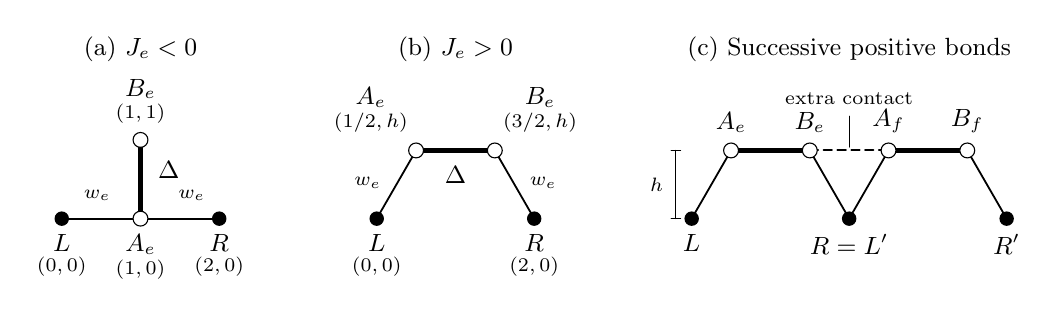
\begin{tikzpicture}[
 x=1cm,y=1cm,line cap=round,
 original/.style={circle,fill=black,draw=black,inner sep=1.7pt},
 ancilla/.style={circle,fill=white,draw=black,inner sep=1.9pt},
 weak/.style={line width=0.65pt},
 strong/.style={line width=1.5pt},
 extra/.style={densely dashed,line width=0.75pt},
 every node/.style={font=\small}]
 \begin{scope}
  \node at (1,2.15) {(a) $J_e<0$};
  \draw[weak] (0,0)--(1,0)--(2,0);
  \draw[strong] (1,0)--(1,1);
  \node[original] at (0,0) {};
  \node[original] at (2,0) {};
  \node[ancilla] at (1,0) {};
  \node[ancilla] at (1,1) {};
  \node[anchor=north] at (0,-0.08)
       {\shortstack{$L$\\[-1pt]\scriptsize$(0,0)$}};
  \node[anchor=north] at (1,-0.08)
       {\shortstack{$A_e$\\[-1pt]\scriptsize$(1,0)$}};
  \node[anchor=north] at (2,-0.08)
       {\shortstack{$R$\\[-1pt]\scriptsize$(2,0)$}};
  \node[anchor=south] at (1,1.08)
       {\shortstack{$B_e$\\[-1pt]\scriptsize$(1,1)$}};
  \node[anchor=west] at (1.10,0.62) {$\Delta$};
  \node[font=\scriptsize,anchor=south] at (0.45,0.10) {$w_e$};
  \node[font=\scriptsize,anchor=south] at (1.65,0.10) {$w_e$};
 \end{scope}
 \begin{scope}[shift={(4,0)}]
  \node at (1,2.15) {(b) $J_e>0$};
  \draw[weak] (0,0)--(0.5,0.8660254);
  \draw[weak] (1.5,0.8660254)--(2,0);
  \draw[strong] (0.5,0.8660254)--(1.5,0.8660254);
  \node[original] at (0,0) {};
  \node[original] at (2,0) {};
  \node[ancilla] at (0.5,0.8660254) {};
  \node[ancilla] at (1.5,0.8660254) {};
  \node[anchor=north] at (0,-0.08)
       {\shortstack{$L$\\[-1pt]\scriptsize$(0,0)$}};
  \node[anchor=north] at (2,-0.08)
       {\shortstack{$R$\\[-1pt]\scriptsize$(2,0)$}};
  \node[anchor=south east] at (0.52,0.97)
       {\shortstack{$A_e$\\[-1pt]\scriptsize$(1/2,h)$}};
  \node[anchor=south west] at (1.48,0.97)
       {\shortstack{$B_e$\\[-1pt]\scriptsize$(3/2,h)$}};
  \node[anchor=north] at (1,0.79) {$\Delta$};
  \node[font=\scriptsize,anchor=east] at (0.18,0.45) {$w_e$};
  \node[font=\scriptsize,anchor=west] at (1.82,0.45) {$w_e$};
 \end{scope}
 \begin{scope}[shift={(8,0)}]
  \node at (2,2.15) {(c) Successive positive bonds};
  \draw[weak] (0,0)--(0.5,0.8660254);
  \draw[weak] (1.5,0.8660254)--(2,0)--(2.5,0.8660254);
  \draw[weak] (3.5,0.8660254)--(4,0);
  \draw[strong] (0.5,0.8660254)--(1.5,0.8660254);
  \draw[strong] (2.5,0.8660254)--(3.5,0.8660254);
  \draw[extra] (1.5,0.8660254)--(2.5,0.8660254);
  \foreach \x in {0,2,4} {\node[original] at (\x,0) {};}
  \foreach \x in {0.5,1.5,2.5,3.5}
       {\node[ancilla] at (\x,0.8660254) {};}
  \node[anchor=north] at (0,-0.08) {$L$};
  \node[anchor=north] at (2,-0.08) {$R=L'$};
  \node[anchor=north] at (4,-0.08) {$R'$};
  \node[anchor=south] at (0.5,0.97) {$A_e$};
  \node[anchor=south] at (1.5,0.97) {$B_e$};
  \node[anchor=south] at (2.5,0.97) {$A_f$};
  \node[anchor=south] at (3.5,0.97) {$B_f$};
  \draw[thin] (-0.2,0)--(-0.2,0.8660254);
  \draw[thin] (-0.26,0)--(-0.14,0);
  \draw[thin] (-0.26,0.8660254)--(-0.14,0.8660254);
  \node[anchor=east,font=\scriptsize] at (-0.24,0.433) {$h$};
  \draw[thin] (2,1.30)--(2,0.91);
  \node[font=\scriptsize,anchor=south] at (2,1.32)
       {extra contact};
 \end{scope}
\end{tikzpicture}
\caption{The contact construction in the local $(\ell,\zeta)$ plane,
with $h=\sqrt3/2$ and $w_e=\sqrt\Delta\,v_e$.
Filled vertices are original spins and open vertices are ancillas.
Every solid segment has length one; thick segments carry weight
$\Delta$ and thin segments the indicated weak weight.  The dashed
segment in (c) is an additional unit contact, with weight zero in
$H_+$; it receives only the small positive hopping floor in the Hubbard
model.  Horizontal gadgets use $\zeta=z$, and vertical gadgets use
$\zeta=-z$.}
\label{fig:gadgets}
\end{figure}

\begin{lemma}[Contact classification]\label{lem:contact-layout}
All the sites $p_i$ are distinct.  Every pair is either at distance one
or at distance at least $\sqrt2$.  The complete set $\mathcal C$ of
unit-distance pairs consists of:
\begin{enumerate}
 \item $L A_e$, $A_e R$, and $A_e B_e$ for a negative source edge;
 \item $L A_e$, $A_e B_e$, and $B_e R$ for a positive source edge;
 \item $B_e A_f$ for two consecutive positive source edges $e,f$ on
       the same original lattice line.
\end{enumerate}
Thus every interaction of $H_+$ is a contact.  Its weight on a contact
will be denoted $K_{ij}\geq0$, using $K_{ij}=0$ for contacts in the
third class.
\end{lemma}

\begin{proof}
Within one gadget the assertion follows directly from
\eqref{eq:gadget-coordinates}.  For a negative gadget the two distances
from $B_e$ to original endpoints are $\sqrt2$; for a positive gadget
the two nonadjacent endpoint--ancilla distances are $\sqrt3$.
Original vertices are mutually separated by at least $2$.
An original vertex other than the endpoints of an ancilla's gadget,
on that same axis line, has along-line distance at least $3/2$ to a
positive ancilla and at least $3$ to a negative midpoint.
An original vertex off that line differs in a transverse coordinate
by at least $2$.

For ancillas belonging to distinct gadgets on the same axis line,
the only along-line separation below $3/2$ is the separation $1$
between $B_e$ and $A_f$ for consecutive positive gadgets.  They have
the same height and hence are a contact.  All remaining such pairs
are at least $3/2>\sqrt2$ apart.  Distinct parallel axis lines have
transverse separation at least $2$.

It remains to compare horizontal and vertical ancillas.  Call an
ancilla \emph{midpoint type} if it belongs to a negative gadget,
and \emph{positive type} otherwise.  Two midpoint-type projections
differ by at least $1$ in each planar coordinate, so their distance
is at least $\sqrt2$.  A midpoint-type and a positive-type projection
differ by at least $1$ and $1/2$ in the two planar coordinates.
Their heights differ by at least $\sqrt3/2$, since horizontal and
vertical heights have opposite signs.  Their squared distance is
therefore at least $1+1/4+3/4=2$.  Finally two positive-type ancillas
from perpendicular directions have height difference $\sqrt3$,
already larger than $\sqrt2$.  These cases exhaust all pairs and
also establish distinctness.
\end{proof}

Orient each contact arbitrarily and write
$u_{ij}=p_j-p_i$, so $|u_{ij}|=1$.  Its first-order length change under
site displacements $s_i$ is $u_{ij}\cdot(s_j-s_i)$.  Reversing the
orientation reverses both factors and leaves this scalar unchanged.
The following stronger-than-counting fact is what permits independent
hopping calibration.

\begin{lemma}[A bounded right inverse for contact lengths]
\label{lem:displacement}
For every real assignment $(d_{ij})_{\{i,j\}\in\mathcal C}$ there
are displacements $s_i\in\mathbb R^3$ such that
\begin{equation}\label{eq:contact-displacement}
 u_{ij}\cdot(s_j-s_i)=d_{ij},\qquad
 \max_i|s_i|\leq6m\max_{\mathcal C}|d_{ij}|.
\end{equation}
For an empty contact set take all displacements zero.  The construction
is linear in $d$, uses polynomially many arithmetic operations with
coefficients in $\mathbb Q(\sqrt3)$, and has no consistency condition
around lattice cycles.
\end{lemma}

\begin{proof}
Set the height displacement of every original vertex to zero.
The horizontal coordinate of each original vertex will be determined
using only its original row, and its vertical planar coordinate using
only its original column.  These are independent variables even when
both directions meet at the same vertex.

Fix one such axis line.  Write $a$ for displacement along it, $z$
for physical height displacement, and put $\sigma=1$ for a horizontal
line and $\sigma=-1$ for a vertical line.  On every connected run of
negative bonds choose the first original $a$ coordinate to be zero,
and accumulate
\begin{equation}\label{eq:negative-displacement}
 \begin{split}
 a_R&=a_L+d_{LA_e}+d_{A_eR},\qquad
 a_{A_e}=a_L+d_{LA_e},\\
 a_{B_e}&=a_{A_e},\qquad
 z_{A_e}=0,\qquad z_{B_e}=\sigma d_{A_eB_e}.
 \end{split}
\end{equation}
Unconstrained original coordinates may be set to zero.  A positive
or missing bond places no requirement on the difference of its
original endpoints' $a$ coordinates at this step, so it separates
runs.  Each run is a path on a line, and
\eqref{eq:negative-displacement} satisfies all three constraints in
its negative gadgets.

Now consider the elevated vertices of positive gadgets on this line.
Their same-height contacts, including the extra contacts of
Lemma~\ref{lem:contact-layout}, form disjoint paths.  Set the first
$a$ coordinate on each path to zero and successively set
$a_{\rm next}=a_{\rm current}+d_{\rm edge}$.
Every such contact vector is along the axis, so its constraint
involves only these $a$ coordinates.  Each elevated vertex has
exactly one additional, sloped contact to an original vertex.
Writing $h_0=\sqrt3/2$, set
\begin{equation}\label{eq:positive-displacement}
 \begin{split}
 z_{A_e}&=\frac{d_{LA_e}-(a_{A_e}-a_L)/2}{\sigma h_0},\\
 z_{B_e}&=\frac{d_{B_eR}-(a_R-a_{B_e})/2}{\sigma h_0}.
 \end{split}
\end{equation}
Indeed the two unit spoke vectors are
$\tfrac12 e_{\rm axis}+\sigma h_0 e_z$ and
$\tfrac12 e_{\rm axis}-\sigma h_0 e_z$, respectively.
Because the original height displacements vanish, these formulas
satisfy the remaining equations without imposing any new condition
on original coordinates.  Set each ancilla's unused transverse
coordinate to zero.

Repeat on all rows and columns.  The row procedure changes only
original $x$ coordinates, and the column procedure only original
$y$ coordinates.  No ancilla belongs to both procedures.  Thus the
constructions do not overwrite each other.  In particular a square
cycle is not a cycle in either scalar accumulation graph; its vector
closure is automatic because actual vertex displacements have been
assigned.

For the norm bound put $d_{\max}=\max_{\mathcal C}|d_{ij}|$.
Every original along-line coordinate has magnitude at most
$2m d_{\max}$, and every accumulated elevated coordinate has
magnitude at most $m d_{\max}$.  Negative ancilla coordinates
have magnitude at most $(2m+1)d_{\max}$ along the line and at
most $d_{\max}$ in height.  From
\eqref{eq:positive-displacement}, positive ancilla heights are at
most $(1+3m/2)d_{\max}/h_0$.  Combining at most two nonzero
coordinates at any site gives the stated bound $6m d_{\max}$.
All assignments are additions and multiplication by fixed rational
numbers or by $1/h_0$, proving the algorithmic assertion.
\end{proof}

Only approximate length equations will be needed.  To make their bit
complexity explicit, suppose the data are known within $\tau/4$ and
apply the displayed right inverse to those approximations.  Approximate
its output and $Dp_i$, then round to rational positions $X_i$, with
total Euclidean error at most $\tau/4$ per site.  Defining
$s_i=X_i-Dp_i$ absorbs this rounding even though the $p_i$ may be
irrational.  Every contact equation then has error at most
$\tau/4+2(\tau/4)<\tau$, and
\begin{equation}\label{eq:rounded-displacement}
 \max_i|s_i|\leq6m\bigl(\max_{\mathcal C}|d_{ij}|+\tau\bigr)+\tau.
\end{equation}
The number of arithmetic operations is polynomial, and all accumulated
coefficients have polynomial size.  Computing $\sqrt3$ and the other
real inputs to sufficiently many additional polynomially bounded bits
therefore gives the stated absolute accuracy in polynomial time.
In particular this does not call for an ill-conditioned general
linear-system solve.

For later use, actual distances satisfy the exact vector identities
and the elementary estimates
\begin{equation}\label{eq:displaced-geometric-bounds}
 \begin{aligned}
 X_j-X_i&=D u_{ij}+s_j-s_i
                       &&(\{i,j\}\in\mathcal C),\\
 |X_j-X_i|&=D+u_{ij}\cdot(s_j-s_i)+O(S^2/D)
                       &&(\{i,j\}\in\mathcal C),\\
 |X_j-X_i|&\geq\sqrt2D-2S
                       &&(\{i,j\}\notin\mathcal C),
 \end{aligned}
\end{equation}
provided $\max_i|s_i|\leq S$ and $S\leq D/4$.  The middle estimate
is the Taylor bound for the Euclidean norm away from zero.  The last
is the triangle inequality and Lemma~\ref{lem:contact-layout}.
No exact nonlinear prescribed-length problem is being solved; the
quadratic remainder will be included in the hopping estimates.

\subsection{The half-filled Hubbard model}

We now realize those positive bonds as second-order hopping processes.
Virtual double occupancy gives the antiferromagnetic superexchange
mechanism of Anderson~\cite{Anderson1959}. In our Pauli-matrix
normalization the coefficient is $t^2/U$ multiplying
$h^s_{ij}-I$. We calculate the fermionic signs below and retain the
constant term, because it contributes to the final decision thresholds.

Associate two fermionic modes, labelled $\uparrow,\downarrow$, to each
of the $m$ sites and restrict to exactly $m$ fermions.  Let
$c_{i\sigma}^\dagger,c_{i\sigma}$ satisfy the canonical
anticommutation relations and put
$n_{i\sigma}=c_{i\sigma}^\dagger c_{i\sigma}$.
For nonnegative hopping strengths define
\begin{equation}\label{eq:hubbard-definition}
 \begin{split}
 H_{\rm Hub}(t)
   &=-\sum_{\{i,j\}\in\mathcal C}\sum_{\sigma=\uparrow,\downarrow}
       t_{ij}\bigl(c_{i\sigma}^\dagger c_{j\sigma}
                  +c_{j\sigma}^\dagger c_{i\sigma}\bigr)
       +U\sum_i n_{i\uparrow}n_{i\downarrow},\\
 U&=\iint_{\mathbb R^3\times\mathbb R^3}
       \frac{\phi(y)^2\phi(y')^2}{|y-y'|}\,\dd y\,\dd y',
       \qquad \phi(y)=\pi^{-1/2}e^{-|y|}.
 \end{split}
\end{equation}
The radial probability density of $\phi^2$ is $p(r)=4r^2e^{-2r}$.
Angular integration gives the kernel $1/\max(r,s)$: for $r,s>0$,
\[
 \frac12\int_{-1}^{1}\frac{\dd u}{\sqrt{r^2+s^2-2rsu}}
      =\frac1{\max(r,s)}.
\]
Since $\int_0^r p(s)\,\dd s=1-e^{-2r}(1+2r+2r^2)$,
\begin{equation}\label{eq:onsite-integral}
 \begin{split}
 U&=8\int_0^\infty r e^{-2r}
           \bigl[1-e^{-2r}(1+2r+2r^2)\bigr]\,\dd r\\
  &=8\left(\frac14-\frac1{16}-\frac1{16}-\frac3{64}\right)
    =\frac58.
 \end{split}
\end{equation}
Thus $U$ is a fixed positive rational constant.

Let $q_{\mathcal C}=|\mathcal C|$ and define the rational scales
\begin{equation}\label{eq:hubbard-scales}
 \overline R=\max\{1,q_{\mathcal C}\Delta\},\qquad
 \eta=\frac{U\gamma}{1024\overline R^3},\qquad
 \alpha=\frac{\eta^2}{U},\qquad
 f=\frac{\alpha\gamma}{128\max\{1,q_{\mathcal C}\}}.
\end{equation}
The ideal hoppings are $t^{(0)}_{ij}=\eta\sqrt{K_{ij}}$.
For each contact compute a rational $r_{ij}$ with
$|r_{ij}-t^{(0)}_{ij}|\leq f$, and output
\begin{equation}\label{eq:hopping-floor}
 t_{ij}=\max\{f,r_{ij}\}.
\end{equation}
Polynomial-precision bisection on nonnegative square roots (at most
two nested square roots here) suffices to compute $r_{ij}$; no exact
comparison between irrational numbers is required.  The maximum in
\eqref{eq:hopping-floor} is a comparison of rationals.  All final
hoppings satisfy $1/\poly(n)\leq t_{ij}<1$, including those with
$K_{ij}=0$.

\begin{proposition}[Hubbard reduction with rational hoppings]
\label{prop:hubbard}
The construction above is deterministic and polynomial time.  With
\begin{equation}\label{eq:finite-scalar-shift}
 C_s=C_0+\sum_{\{i,j\}\in\mathcal C}K_{ij}
     =3k\Delta+\frac32\sum_e v_e^2
                        +\sum_{\{i,j\}\in\mathcal C}K_{ij},
\end{equation}
it satisfies
\begin{equation}\label{eq:finite-combined-error}
 \left|E\bigl(H_{\rm Hub}(t)\bigr)
            -\alpha\bigl(E(H_{\rm in})-C_s\bigr)\right|
        \leq\frac{3\alpha\gamma}{64}.
\end{equation}
The scalar $C_s$ has polynomial magnitude and can be approximated to
any polynomial-bit absolute precision in polynomial time.
\end{proposition}

\begin{proof}
First use the ideal hoppings $t^{(0)}$.  Let
$A_U=U\sum_i n_{i\uparrow}n_{i\downarrow}$ and let $T$ be the hopping
part of $H_{\rm Hub}(t^{(0)})$.  At filling $m$, the kernel of $A_U$
is exactly the singly occupied subspace: having $m$ fermions, at most
one at each of $m$ sites, forces precisely one per site.  Identify this
subspace with $m$ spins, and denote its projection by $P_{\rm so}$.
The complementary excitation energies are positive integer multiples
of $U$.  A single hop from $P_{\rm so}$ creates one vacant site
and one doubly occupied site and hence has energy exactly $U$.
In particular $P_{\rm so}TP_{\rm so}=0$.

A second hop can return to single occupancy only by moving an electron
from that doubly occupied site to that vacant site.  Thus the two hops
must use the same unordered bond; products from different bonds have
zero compression, even when the bonds share a vertex.
For completeness, consider one bond $i,j$ of strength $t$, with local
mode order $i\uparrow,i\downarrow,j\uparrow,j\downarrow$.
Write $|D_i\rangle=c_{i\uparrow}^\dagger
c_{i\downarrow}^\dagger|0\rangle$ and similarly for $|D_j\rangle$.
The bond hopping operator $T_{ij}$ obeys
\[
 T_{ij}|\uparrow,\downarrow\rangle
      =-t(|D_i\rangle+|D_j\rangle),\qquad
 T_{ij}|\downarrow,\uparrow\rangle
      = t(|D_i\rangle+|D_j\rangle).
\]
It consequently annihilates all triplets and maps the singlet to
$-\sqrt2t(|D_i\rangle+|D_j\rangle)$, of squared norm $4t^2$.
In an ordering containing other sites between $i$ and $j$, those sites
are singly occupied during this two-hop process; their fixed fermion
parity changes transition phases but not the compressed product.
Equivalently, permuting the intervening mode pairs gives the same
calculation under a fermionic change of basis.  It follows that
\begin{equation}\label{eq:hubbard-exchange}
 -P_{\rm so}T_{ij}A_U^{-1}T_{ij}P_{\rm so}
       =-\frac{4t^2}{U}P_{{\rm singlet},ij}
       =\frac{t^2}{U}(h^s_{ij}-I).
\end{equation}
Here $P_{{\rm singlet},ij}=(I-h^s_{ij})/4$.

For each spin, $c_{i\sigma}^\dagger c_{j\sigma}
+c_{j\sigma}^\dagger c_{i\sigma}$ has norm one, so
\[
 \lVert T\rVert\leq2\sum_{\mathcal C}t^{(0)}_{ij}
       =2\eta\sum_{\mathcal C}\sqrt{K_{ij}}
       \leq2\eta\overline R.
\]
The last inequality uses $K_{ij}\leq\Delta$ and $\Delta\geq1$.
Lemma~\ref{lem:second-order}, with $g=U$ and
$\epsilon=2\eta\overline R/U<1/2$, and
\eqref{eq:hubbard-exchange} give
\begin{equation}\label{eq:ideal-hubbard-error}
 \left|E\bigl(H_{\rm Hub}(t^{(0)})\bigr)
       -\alpha\left(E(H_+)-\sum_{\mathcal C}K_{ij}\right)\right|
 \leq\frac{16\eta^3\overline R^3}{U^2}
 \leq\frac{\alpha\gamma}{64}.
\end{equation}
If the complementary subspace is empty, as can happen for $m=1$,
there is no hopping and this assertion is exact.

For the rational hoppings, nonnegativity of $t^{(0)}_{ij}$ and the
accuracy of $r_{ij}$ imply
$|\max\{f,r_{ij}\}-t^{(0)}_{ij}|\leq f$.
Therefore
\begin{equation}\label{eq:hopping-rounding-error}
 \left\|H_{\rm Hub}(t)-H_{\rm Hub}(t^{(0)})\right\|
      \leq2q_{\mathcal C}f\leq\frac{\alpha\gamma}{64}.
\end{equation}
Also $t^{(0)}_{ij}\leq\eta\overline R\leq U/1024$ and
$f\leq U/(128\cdot1024^2)$, which verify $f\leq t_{ij}<1$.
The floor $f$ is an inverse polynomial.  This argument covers an ideal
hopping much smaller than $f$ and an ideal hopping equal to zero; no
coefficient lower bound has been used.  If $\mathcal C$ is empty,
\eqref{eq:hopping-rounding-error} is simply zero.

Finally, Proposition~\ref{prop:positive-spin} with
\eqref{eq:spin-scale} contributes at most another
$\alpha\gamma/64$.  Adding the three errors proves
\eqref{eq:finite-combined-error}.  All sizes, magnitudes, and reciprocal
precision budgets in the construction are polynomial in $n$.
Each $K_{ij}$ is either $\Delta$, a square root of the rational number
$2\Delta|J_e|$, or zero.  The displayed scalar shift is thus efficiently
approximable to the asserted precision, completing the proof.
\end{proof}

\section{Isolated wells and deterministic energy tuning}
\label{sec:wells}

This section supplies an exponentially accurate classical procedure for
tuning the individual well energies. The procedure operates on
one-electron operators only; it does not diagonalize any of the spin or
Hubbard Hamiltonians from \Cref{sec:finite}.

There are two separate tasks. First we must show that moving a secondary
positive nucleus changes one isolated energy monotonically, with much
weaker effects on the other sites. Then we must evaluate those energies
accurately enough to implement the resulting contraction. The required
accuracy is exponential in $D$: an inverse-polynomial energy error in
these dilated units would grow after the final amplification. The
analytic and arithmetic estimates below address that precision cost.

Fix centers \(X_1,\ldots,X_m\in\R^3\) satisfying
\begin{equation}
 |X_i-X_j|\ge D-2S\quad(i\ne j),\qquad S\le D/100.
 \label{eq:wells-separation}
\end{equation}
Here \(D\) is a sufficiently large integer and \(m/D\) is smaller than a
sufficiently small absolute constant. All constants in this section are
uniform in the centers and the parameters \(\rho_i\in[1,4]\).
The stronger scale requirements used later imply these hypotheses.
Computational statements additionally assume rational centers. Their
bit lengths, rather than their numerical magnitudes, enter the
complexity bounds.

Choose an integer \(Z_*\) with \(e^D/2\le Z_*\le2e^D\). Round the following
two numbers to nearest integers, once and for all, before tuning:
\begin{equation}
\begin{split}
 Z_*q&=\operatorname{round}\!\left(
              Z_*\left(1-\frac{500m}{D}\right)\right),\\
 Z_*q'&=\operatorname{round}\!\left(Z_*\frac{1000m}{D}\right).
\end{split}
 \label{eq:wells-charges}
\end{equation}
Both integers are positive for the scales considered here. In particular,
\begin{equation}
\begin{split}
 q&=1-\frac{500m}{D}+O(Z_*^{-1}),\\
 q'&=\frac{1000m}{D}+O(Z_*^{-1}),\qquad
 c\frac mD\le q'\le C\frac mD.
\end{split}
 \label{eq:wells-charge-bounds}
\end{equation}
The primary and secondary nuclei of site \(i\) are at \(X_i\) and
\(X_i+\rho_i e_z\), respectively, in scaled coordinates. Write
\begin{equation}
\begin{split}
 r_i&=|y-X_i|,\qquad
 V_i(y)=\frac q{r_i}+\frac{q'}{|y-X_i-\rho_i e_z|},\\
 h&=-\frac12\Delta-\sum_{i=1}^m V_i.
\end{split}
 \label{eq:wells-full-one-body}
\end{equation}
These are the one-electron operators obtained from physical coordinates
by \(y=Z_*x\) and division of energies by \(Z_*^2\).

Fix a nondecreasing \(C^2\) function \(\chi:[0,\infty)\to[0,1]\) that
vanishes on \([0,1/16]\) and equals one on \([1/8,\infty)\). It can have
rational piecewise-polynomial data: integrate a normalized positive
multiple of \((t-1/16)^2(1/8-t)^2\) on the transition interval and extend
constantly outside. Set
\begin{equation}
 \chi_i(y)=\chi(r_i/D),\qquad
 W_i=\sum_{k\ne i}\chi_k V_k,\qquad
 h_i=-\frac12\Delta-V_i-W_i.
 \label{eq:wells-capped}
\end{equation}
The caps remove the other nuclear singularities from \(h_i\) while
retaining their fields near site \(i\).

\subsection{Uniform ground-state estimates}

We use the three-dimensional Sobolev bounds
\(\|u\|_6\le C\|u\|_{H^1}\) and
\(\|u\|_\infty\le C\|u\|_{H^2}\), together with their localized versions.
We also use the translated Hardy inequality
\begin{equation}
 \left\|\frac{u}{|\,\cdot-a\,|}\right\|_2
 \le2\|\nabla u\|_2\qquad(a\in\R^3).
 \label{eq:wells-hardy}
\end{equation}
Indeed, integrate
\(\operatorname{div}((y-a)/|y-a|^2)=|y-a|^{-2}\)
against \(|u|^2\) for a smooth compactly supported \(u\). Integration by
parts and Cauchy--Schwarz give
\[
 \|u/|\,\cdot-a\,|\|_2^2
 \le2\|u/|\,\cdot-a\,|\|_2\|\nabla u\|_2.
\]
Approximation proves \eqref{eq:wells-hardy} on \(H^1\).
Thus Coulomb multiplication maps \(H^1\) continuously into \(L^2\),
uniformly in the location of the pole.

\begin{proposition}[Uniform isolated-well estimates]
\label{prop:isolated-well}
The operators \(h_i\) are self-adjoint on \(H^2(\R^3)\), with form domain
\(H^1(\R^3)\). Each has a simple ground eigenvalue \(\lambda_i\) and a
real, positive, normalized eigenfunction \(\psi_i\). There is a constant
\(g>0\) such that the remaining spectrum is at least \(\lambda_i+g\).
For \(\phi_i(y)=\pi^{-1/2}e^{-r_i}\),
\begin{equation}
 |\lambda_i+1/2|\le C\frac mD,\qquad
 \|\psi_i-\phi_i\|_{H^2}\le C\frac mD.
 \label{eq:wells-h2}
\end{equation}
Moreover, for derivative orders \(j=0,1,2\),
\begin{equation}
 \|D^jW_i\|_\infty\le C\frac m{D^{j+1}},
 \qquad 0\le W_i\le\frac{100m}{D}.
 \label{eq:wells-field-bounds}
\end{equation}
These assertions hold before tuning and uniformly throughout
\([1,4]^m\).
\end{proposition}

\begin{proof}
On the nonzero support of \(\chi_k\), \(r_k\ge D/16\). Since \(\rho_k\le4\),
\[
 |y-X_k-\rho_k e_z|\ge r_k-4\ge r_k/2
\]
for large \(D\). The secondary singularity is inside the region where
the cap is identically zero. Differentiation through order two,
including derivatives of the cap, gives
\(\|D^j(\chi_kV_k)\|_\infty\le CD^{-j-1}\).
Summing proves the derivative bounds. For example, \(q\le1\), \(q'\le1\),
and sufficiently large \(D\) give a bound below \(100/D\) for each capped
potential, proving the stated function bound.

Put \(H_i^0=-\Delta/2-r_i^{-1}\) and \(B_i=h_i-H_i^0\).
Hardy's inequality and \eqref{eq:wells-field-bounds} give
\begin{equation}
 \|B_i u\|_2\le C\frac mD\|u\|_{H^1}.
 \label{eq:wells-perturbation}
\end{equation}
For any potential in these single-well operators, Hardy and Fourier
interpolation give, for each \(a>0\), a uniform bound
\(\|Vu\|_2\le a\|\Delta u\|_2+C_a\|u\|_2\).
The Kato--Rellich theorem for relatively bounded perturbations
\cite[Theorem~6.4, p.~135]{Teschl2009} therefore gives domain \(H^2\). The same estimates, with the Laplacian term
absorbed, prove uniform graph-norm equivalence:
\begin{equation}
 C^{-1}\|u\|_{H^2}
 \le \|h_i u\|_2+C\|u\|_2
 \le C\|u\|_{H^2}.
 \label{eq:wells-graph-norm}
\end{equation}
The corresponding statement holds for \(H_i^0\).
At form level a fixed positive shift of either operator is bounded
above and below by constant multiples of \(\|u\|_{H^1}^2\), giving
the asserted form domains.

The hydrogenic ground state and its isolation follow without an
excited-state formula. Direct integration by parts gives
\begin{equation}
 \langle u,(H_i^0+1/2)u\rangle
 =\frac12\left\|\nabla u+\frac{y-X_i}{r_i}u\right\|_2^2.
 \label{eq:wells-hydrogen-square}
\end{equation}
Its zero vectors are exactly the multiples of \(\phi_i\).
If normalized vectors orthogonal to \(\phi_i\) had energies tending to
\(-1/2\), they would be bounded in \(H^1\). The Coulomb form is compact
under weak convergence of such a sequence: within radius \(a\) of the
pole its absolute value is bounded by \(Ca\|u\|_{H^1}^2\), by Sobolev and
H\"older; beyond radius \(R\) it is bounded by \(R^{-1}\|u\|_2^2\);
on the intervening annulus local compactness applies. A weak limit
would therefore obey
\[
 \langle u,H_i^0u\rangle\le-1/2,\qquad
 \langle u,H_i^0u\rangle\ge-\tfrac12\|u\|_2^2\ge-1/2.
\]
Equality forces norm one and a multiple of \(\phi_i\), contrary to
orthogonality. This proves a fixed gap \(g_0>0\).

By \eqref{eq:wells-perturbation}, after a fixed positive shift the
perturbed form lies between \(1-Cm/D\) and \(1+Cm/D\) times the
unperturbed shifted form. The variational principle puts its first
level within \(Cm/D\) of \(-1/2\), and its second variational level at
least \(-1/2+g_0-Cm/D\). The negative first level is attained.
The preceding truncation argument gives form compactness of both own
Coulomb potentials and of the bounded decaying \(W_i\). A normalized
minimizing sequence is bounded in \(H^1\). Passing to a weakly convergent
subsequence with limit \(u\), compactness and lower semicontinuity give
\[
 \lambda_i\|u\|_2^2\le\langle u,h_i u\rangle\le\lambda_i<0.
\]
Since \(\|u\|_2\le1\), these inequalities force \(\|u\|_2=1\)
and attainment. For small enough \(m/D\) the
first level is simple and separated from the rest by a fixed \(g>0\).
Taking the absolute value of a real minimizer cannot increase its
energy. The Euler equation and the strong maximum principle on the
connected complement of the poles make it positive there.

The form bounds give \(\|\psi_i\|_{H^1}\le C\). Its equation implies
\[
 (H_i^0+1/2)\psi_i
   =(\lambda_i+1/2)\psi_i-B_i\psi_i,
\]
with right side of norm at most \(Cm/D\). On \(\phi_i^\perp\), the inverse
of \(H_i^0+1/2\) is bounded from \(L^2\) to \(H^2\): use the gap for the
\(L^2\) bound, then \eqref{eq:wells-graph-norm}.
The orthogonal component of \(\psi_i\) consequently has \(H^2\) norm
\(O(m/D)\). Normalization and the positive overlap with \(\phi_i\) put
its coefficient along \(\phi_i\) within \(O((m/D)^2)\) of one.
This proves \eqref{eq:wells-h2} and the uniform sup bound. Positivity
also holds at the poles by continuity and this sup-norm approximation,
since both poles lie within distance four of \(X_i\).
\end{proof}

\subsection{Moving the secondary nucleus}

The derivative of a moving Coulomb potential is not an \(L^2\)-bounded
multiplier. We instead control its expectations by Hardy's inequality.

\begin{lemma}[Bracketing and uniform secant bounds]
\label{lem:wells-secants}
With centers and rounded charges fixed, for every choice of the other
parameters,
\(\lambda_i(\rho_i=1)<-1/2<\lambda_i(\rho_i=4)\).
For \(1\le a<b\le4\), holding the other parameters fixed,
\begin{equation}
 c q'(b-a)\le\lambda_i(b)-\lambda_i(a)\le Cq'(b-a).
 \label{eq:wells-own-slope}
\end{equation}
If instead \(\rho_i\) is held fixed, then
\begin{equation}
 |\lambda_i(\rho)-\lambda_i(\widetilde\rho)|
 \le Cq'\frac m{D^2}\|\rho-\widetilde\rho\|_\infty.
 \label{eq:wells-other-slope}
\end{equation}
\end{lemma}

\begin{proof}
Taking the inner product of the eigen-equation with \(\phi_i\) gives
\begin{equation}
 \lambda_i=-\frac12+(1-q)-q'f(\rho_i)
       -\langle\phi_i,W_i\phi_i\rangle+O((m/D)^2),
 \label{eq:wells-energy-expansion}
\end{equation}
where
\[
 f(\rho)=\int_{\R^3}\frac{\pi^{-1}e^{-2|y|}}{|y-\rho e_z|}\dd y.
\]
Here \(\langle\phi_i,\psi_i\rangle=1+O((m/D)^2)\), and replacing
\(\psi_i\) by \(\phi_i\) in a perturbing expectation costs \(O((m/D)^2)\),
by \eqref{eq:wells-perturbation} and \eqref{eq:wells-h2}.
Also \(\langle\phi_i,r_i^{-1}\phi_i\rangle=1\).
The spherical average of \(|r\omega-\rho e_z|^{-1}\) is
\(1/\max(r,\rho)\), as direct integration in \(\omega\cdot e_z\) shows.
Consequently,
\begin{align}
 f(\rho)&=\rho^{-1}\int_0^\rho4r^2e^{-2r}\dd r
             +\int_\rho^\infty4r e^{-2r}\dd r,
 \label{eq:wells-radial-potential}\\
 f'(\rho)&=-\rho^{-2}\int_0^\rho4r^2e^{-2r}\dd r.
 \label{eq:wells-f-derivative}
\end{align}
In particular,
\[
 f(1)=1-2e^{-2}>0.7,\quad f(4)\le\tfrac14,\quad
 \frac{1-5e^{-2}}{16}\le-f'(\rho)\le1\quad(1\le\rho\le4).
\]
At the first endpoint the leading shift in
\eqref{eq:wells-energy-expansion} is at most \((500-700)m/D\);
at the second it is at least \((500-250-100)m/D\).
The quadratic and rounding errors fit inside these strict margins,
proving bracketing.

For the secant bound, fix a ground function \(u\) at either endpoint,
and put \(A(t)=X_i+t e_z\). The kernel derivative is dominated by
\(|y-A(t)|^{-2}\), and Hardy gives
\begin{align}
 \int\frac{|u^2-\phi_i^2|}{|y-A(t)|^2}\dd y
 &\le\left\|\frac{u-\phi_i}{|\,\cdot-A(t)\,|}\right\|_2
       \left\|\frac{u+\phi_i}{|\,\cdot-A(t)\,|}\right\|_2 \notag\\
 &\le4\|\nabla(u-\phi_i)\|_2
       \bigl(\|\nabla u\|_2+\|\nabla\phi_i\|_2\bigr)
 \le C\frac mD.
 \label{eq:wells-density-hardy}
\end{align}
The same bound with \(u^2\) justifies absolute integration in \(y\)
and \(t\). Thus replacing the density by \(\phi_i^2\) when integrating
the moving-pole kernel derivative incurs at most
\(Cq'(m/D)(b-a)\) error.
The variational principle gives
\[
 \langle\psi_i(b),(h_i(b)-h_i(a))\psi_i(b)\rangle
 \le\lambda_i(b)-\lambda_i(a)
 \le\langle\psi_i(a),(h_i(b)-h_i(a))\psi_i(a)\rangle.
\]
Both bounding quantities differ from \(-q'(f(b)-f(a))\) by the error
just estimated, proving \eqref{eq:wells-own-slope}.

For \(k\ne i\), the moving secondary pole in \(\chi_kV_k\) stays at
least \(D/32\) from the region where its cap is nonzero.
Its bounded potential changes in sup norm by at most
\(Cq'D^{-2}|\rho_k-\widetilde\rho_k|\).
Summing and applying the variational principle for a bounded additive
perturbation proves \eqref{eq:wells-other-slope}.
\end{proof}

\Needspace{10\baselineskip}
\subsection{Uniform tails}

\begin{lemma}[Crude tails before tuning]
\label{lem:well-tail}
Uniformly for all \(\rho\in[1,4]^m\),
\begin{equation}
 |\psi_i(y)|\le C\exp[-.99(r_i-.01D)],
 \label{eq:wells-tail}
\end{equation}
and, for sufficiently large \(D\),
\begin{equation}
 \|\psi_i\|_{H^1(\{r_i>.65D\})}\le e^{-.61D}.
 \label{eq:wells-h1-tail}
\end{equation}
\end{lemma}

\begin{proof}
On \(r_i\ge .01D\), both own poles are far away and
\(V_i+W_i=O(m/D)\). For \(a=.99\) and
\(b(y)=C\exp[-a(r_i-.01D)]\), direct calculation gives
\[
 \frac{(h_i-\lambda_i)b}{b}
 =-\frac{a^2}{2}+\frac a{r_i}-V_i-W_i-\lambda_i.
\]
Its constant part is \((1-a^2)/2+O(m/D)>0\) at the chosen scales.
The zero-order coefficient of \(h_i-\lambda_i\) is also positive
throughout this exterior region. The uniform sup bound fixes \(C\)
so that \(b\ge|\psi_i|\) at the inner boundary. An \(H^2(\R^3)\) function
is uniformly continuous and vanishes at infinity; otherwise uniform
continuity on a sequence of disjoint balls would contradict its
square integrability. On a large finite annulus add a constant
\(\varepsilon>0\) to \(b\) to dominate both signs of \(\psi_i\) at the
outer boundary. The supersolution inequality is preserved.
Testing the negative part of \(b+\varepsilon\mp\psi_i\) proves
comparison. Send the outer radius to infinity and then
\(\varepsilon\) to zero. Inside \(.01D\), the same sup bound proves
\eqref{eq:wells-tail}.

For the gradient estimate choose a smooth cutoff \(\zeta\) that vanishes
on \(r_i\le .645D\), equals one on \(r_i\ge .65D\), and has gradient
\(O(D^{-1})\). Testing the eigen-equation with \(\zeta^2\psi_i\) gives
\[
 \frac12\|\nabla(\zeta\psi_i)\|_2^2
 =\int(V_i+W_i+\lambda_i)|\zeta\psi_i|^2\dd y
       +\frac12\int|\nabla\zeta|^2|\psi_i|^2\dd y.
\]
All coefficients on this support are bounded. Thus
\eqref{eq:wells-tail} bounds the exterior \(H^1\) norm by a polynomial in
\(D\) times \(\exp[-.99(.645-.01)D]\).
Since \(.99(.645-.01)=.62865>.61\), the polynomial factor is absorbed
for large \(D\).
\end{proof}

\subsection{An analytic estimate with uniform constants}

We give the local regularity argument used in the numerical procedure.
It explains why the shrinking length scales near a moving Coulomb pole
do not increase the required polynomial degree beyond \(O(D)\).

\begin{lemma}[Uniform analytic patches]
\label{lem:wells-analytic}
Suppose \(u\) is bounded on the unit ball in \(\R^3\) and satisfies
\(\Delta u=Fu\) there, where
\begin{equation}
 \|\partial^\beta F\|_\infty\le A^{|\beta|+1}|\beta|!
 \quad\text{for every multi-index }\beta.
 \label{eq:wells-analytic-coefficient}
\end{equation}
There is a constant \(A_1\), depending only on \(A\), such that
\begin{equation}
 \max_{|\alpha|=k}\|\partial^\alpha u\|_{L^\infty(B_{1/4})}
 \le \|u\|_{L^2(B_1)}A_1^{k+1}k!.
 \label{eq:wells-analytic-derivatives}
\end{equation}
On a sufficiently small fixed ball about the origin, Taylor
polynomials consequently have geometrically decreasing errors in
both value and first derivative, with constants depending only on \(A\).
\end{lemma}

\begin{proof}
For two concentric balls of radii between \(1/2\) and \(1\), separated
by \(h\), the local estimates needed below are
\begin{align}
 \|D^2v\|_{2,\mathrm{inner}}
 &\le C\bigl(\|\Delta v\|_{2,\mathrm{outer}}
                   +h^{-2}\|v\|_{2,\mathrm{outer}}\bigr),
 \label{eq:wells-local-h2}\\
 \|\nabla v\|_{2,\mathrm{inner}}
 &\le C\bigl(h\|\Delta v\|_{2,\mathrm{outer}}
                   +h^{-1}\|v\|_{2,\mathrm{outer}}\bigr).
 \label{eq:wells-local-h1}
\end{align}
To obtain them, insert smooth cutoffs with first and second derivatives
\(O(h^{-1})\) and \(O(h^{-2})\). Integration by parts against a squared
cutoff and Cauchy--Schwarz, with \(ab\le (h a)^2/2+(b/h)^2/2\),
bound first derivatives on an intermediate ball as in
\eqref{eq:wells-local-h1}. Apply the whole-space Fourier inequality
\(\|D^2w\|_2\le C\|\Delta w\|_2\) to the cutoff function and substitute
that first-derivative bound in its commutator terms to obtain
\eqref{eq:wells-local-h2}. Approximation proves these estimates for
weak solutions. Successive localized Laplacian regularity makes \(u\)
smooth when \(F\) is smooth, justifying the following differentiations.

Fix an integer \(\ell\ge2\), set \(r_j=1-j/(2\ell)\), and write
\[
 T_j=\max_{|\alpha|=j}\|\partial^\alpha u\|_{L^2(B_{r_j})},
 \qquad M=\|u\|_{L^2(B_1)}.
\]
The first-derivative bound gives \(T_1\le C(\ell+A/\ell)M\).
For \(j\le\ell-2\), apply \eqref{eq:wells-local-h2} to an order-\(j\)
derivative between \(B_{r_j}\) and \(B_{r_{j+2}}\).
Leibniz' rule yields
\begin{equation}
 T_{j+2}\le C\left(
  \sum_{b=0}^j\binom jb A^{b+1}b!\,T_{j-b}
  +\ell^2T_j\right).
 \label{eq:wells-analytic-recurrence}
\end{equation}
Lower-order derivatives are available on the larger balls
\(B_{r_{j-b}}\). The multi-index coefficient sum of order \(b\)
is \(\binom jb\), by the multinomial identity.
If preceding orders satisfy \(T_s\le M(K\ell)^s\), the sum is at most
\[
 AM(K\ell)^j\sum_{b=0}^j(A/K)^b
 \le2AM(K\ell)^j
\]
for \(K\ge2A\), using \(\binom jb b!\le\ell^b\).
Increasing the fixed \(K\) absorbs the remaining \(C\ell^2\) factor
into \((K\ell)^2\). Both parity chains therefore satisfy
\(T_j\le M(K\ell)^j\).

Set \(\ell=k+2\). Sobolev embedding on fixed smaller balls bounds the
sup norm of an order-\(k\) derivative on \(B_{1/4}\) by
\(CM[K(k+2)]^{k+2}\).
The inequality \(k!\ge(k/e)^k\), with the small cases absorbed in
the constant, converts this into \eqref{eq:wells-analytic-derivatives}.
Taylor's formula, summed over multi-indices, bounds the degree-\(L\)
remainder on \(|z|\le a\) by a constant times \((C_1a)^{L+1}\).
The first-derivative remainder has an additional factor polynomial
in \(L\) and the same geometric decay. Fixing \(a\) small enough that
\(C_1a<1\) proves the last assertion.
\end{proof}

\subsection{A polynomial-size graded Ritz space}

Graded meshes with increasing polynomial degree are a standard way to
combine singular local behavior with exponential approximation away from
the singularities. For related eigenvalue approximation results with
singular potentials, see Maday and Marcati~\cite{MadayMarcati2019}.
Their bounded-domain discontinuous-Galerkin estimates are not an oracle
for the present moving attractive Coulomb wells. We construct the needed
conforming space and then certify its matrix arithmetic separately.
More specifically, the products of tensor-linear hats with local
polynomials below form a partition-of-unity approximation space, as in
Melenk and Babu\v{s}ka~\cite[Section~2]{MelenkBabuska1996}.
We give the cutoff and derivative estimates explicitly because the tensor
cells can have arbitrarily large aspect ratios.

This is a form-domain approximation: the piecewise polynomial
functions need only belong to \(H^1\). Their kinetic matrix uses first
weak derivatives, not second derivatives across element boundaries.

\begin{lemma}[Exponentially accurate Ritz approximation]
\label{lem:wells-ritz-approximation}
For each \(i\), each rational choice of centers and secondary parameters,
and each sufficiently large \(D\), one can explicitly construct a space
\(\mathcal V_i\subset H^1(\R^3)\) of rational piecewise polynomials,
of dimension polynomial in \(D\), supported in \(r_i<.8D\), such that
\begin{equation}
 \inf_{v\in\mathcal V_i}\|v-\psi_i\|_{H^1}\le e^{-.58D}.
 \label{eq:wells-ritz-h1}
\end{equation}
Its lowest Ritz value \(\lambda_i^{\mathrm R}\) satisfies
\begin{equation}
 0\le\lambda_i^{\mathrm R}-\lambda_i\le C e^{-1.16D}.
 \label{eq:wells-ritz-bias}
\end{equation}
The construction and constants are uniform over rational parameters
throughout \([1,4]^m\).
\end{lemma}

\begin{proof}
Work in local coordinates \(z=y-X_i\) on \([-D,D]^3\), with poles
at \(0\) and \(\rho_i e_z\). Put \(\delta=2^{-8D}\) and fix a sufficiently
small rational \(\xi>0\), as specified below. On each coordinate axis
let \(B\) be the set of projections of the two poles. Starting from
\([-D,D]\), bisect dyadically until every interval \(I\) obeys
\begin{equation}
 |I|\le\xi\min\{1,\dist(I,B)+\delta\}.
 \label{eq:wells-grid-rule}
\end{equation}
Every leaf length is at least \(\xi\delta/2\), since its parent failed
the stopping rule. Above a fixed spacing there are \(O(D)\) intervals.
At a finer level of length \(h\), only intervals within \(h/\xi\) of
one of the at most two projections can still split, so a fixed number
of intervals per level are split there.
There are \(O(\log(D/\delta))=O(D+\log D)\) levels, hence \(O(D)\)
intervals per axis. This remains true for poles arbitrarily close to
dyadic boundaries. The tensor product has \(O(D^3)\) nodes and cells.

Let \(b_w\) be the tensor-linear hat at node \(w\). The full hats form
a partition of unity in the cube. Retain nodes satisfying
\begin{equation}
 |w|<.73D,\qquad |w|>\delta,\qquad
 |w-\rho_i e_z|>\delta,
 \label{eq:wells-retained-nodes}
\end{equation}
and take \(b_w(z)(z-w)^\alpha\) for all \(|\alpha|\le L_0\), where \(L_0\)
is a sufficiently large fixed multiple of \(D\). These functions span
\(\mathcal V_i\), whose dimension before removing dependencies is
\(O(D^6)\).

Here is the support estimate that avoids any aspect-ratio assumption.
For either pole \(a\), every coordinate interval adjacent to \(w\) obeys
\[
 |I|\le\xi\min\{1,|w_j-a_j|+\delta\}.
\]
The support radius \(R_w^{\mathrm{hat}}\) of a retained hat thus satisfies
\begin{equation}
\begin{split}
 R_w^{\mathrm{hat}}
 &\le\xi\bigl(|w-a|+\sqrt3\delta\bigr)
   \le(1+\sqrt3)\xi|w-a|,\\
 R_w^{\mathrm{hat}}&\le\sqrt3\xi.
\end{split}
 \label{eq:wells-patch-radius}
\end{equation}
For \(d_w=\min\{1,|w|,|w-\rho_i e_z|\}\) this gives
\(R_w^{\mathrm{hat}}\le C\xi d_w\). Each support avoids both poles and,
for large \(D\), lies in \(|z|<.8D\).

Choose a fixed \(c<1/10\) and set \(R=c d_w\).
The whole ball \(B(w,R)\) avoids both poles. Throughout it every remote
primary has distance at least \(D-2S-.73D-c>D/8\), so it also avoids
every remote cap transition. On this enlarged ball the eigen-equation
contains only pure Coulomb potentials. Rescaling by \(R\) gives
\(\Delta u=Fu\) on the unit ball. Its coefficient satisfies
\eqref{eq:wells-analytic-coefficient} with an absolute \(A\):
local inverse-distance expansions give factorial derivative bounds
because \(R/\dist(w,a)\le c\); the extra \(R^2\) in the coefficient
makes \(R^2/\dist(w,a)\) bounded; and remote contributions sum to at
most \(Cm/D\). The eigenvalue term is bounded too.
The sup norm of \(u\) is uniform by \Cref{prop:isolated-well}.

Choose \(\xi\) sufficiently small compared to \(c\) and the fixed
analytic radius in \Cref{lem:wells-analytic}, putting the hat supports
inside that smaller ball after rescaling. With \(L_0\) a sufficiently
large fixed multiple of \(D\), its Taylor polynomial \(p_w\) satisfies
\begin{equation}
 |\psi_i-p_w|+R|\nabla\psi_i-\nabla p_w|\le e^{-20D}
 \quad\text{on }\supp b_w.
 \label{eq:wells-taylor-error}
\end{equation}
Increasing the fixed multiple absorbs the polynomial factor in the
differentiated remainder. The Taylor coefficients establish existence
of an approximant; the algorithm will not compute them.

To remove tiny neighborhoods of the poles and the exterior, let
\(a_{\mathrm{out}}\) equal one up to radius \(.66D\), decrease linearly
to zero by \(.72D\), and vanish thereafter. Let \(a_{\mathrm{in}}\) vanish
up to \(\delta\), increase linearly to one by \(2\delta\), and equal one
thereafter. Sample
\[
 a_{\mathrm{out}}(|z|)\,
 a_{\mathrm{in}}(|z|)\,
 a_{\mathrm{in}}(|z-\rho_i e_z|)
\]
at all grid nodes to get weights \(c_w\in[0,1]\), and put
\(b=\sum_w c_wb_w\). Nonzero weights occur only at retained nodes.
The function \(b\) equals one away from \(O(\delta)\)-balls about the
poles and away from \(|z|>.65D\): a node within \(2\delta\) of a pole
has adjacent lengths \(O(\xi\delta)\), whereas all intervals have
length at most \(\xi\). These facts localize the inner and outer
transitions, respectively.

Each first derivative of a tensor-linear interpolant is a convex
combination of edge secants in that coordinate. Consequently
\(|\nabla b|\le C/\delta\) on the inner transitions and
\(|\nabla b|\le C/D\) on the outer transition, irrespective of aspect
ratios. The bounded sup norm of \(\psi_i\) makes the inner
cutoff-gradient cost \(C\delta^{1/2}\). Also, by its \(H^2\) bound,
\[
 \|\nabla\psi_i\|_{L^2(B_{C\delta}(a))}
 \le C\delta\|\nabla\psi_i\|_6\le C\delta.
\]
The exterior cost follows from \eqref{eq:wells-h1-tail}. Thus
\begin{equation}
 \|\psi_i-b\psi_i\|_{H^1}
 \le C\bigl(\sqrt\delta+e^{-.61D}\bigr).
 \label{eq:wells-cutoff-error}
\end{equation}
The cutoff weights, like the Taylor coefficients, are only existence
coefficients in the explicitly generated space.

Set \(v=\sum_w c_wb_wp_w\in\mathcal V_i\).
At almost every point at most eight hats are nonzero. Their derivatives
cost at most \(C/\delta\), by the minimum interval length, and
\(R^{-1}\le C/\delta\).
On a region of volume \(O(D^3)\), \eqref{eq:wells-taylor-error} gives
\[
 \|b\psi_i-v\|_{H^1}\le C D^{3/2}\delta^{-1}e^{-20D}.
\]
Since \(\sqrt\delta=e^{-4(\log2)D}\) and
\(\delta^{-1}e^{-20D}=e^{-(20-8\log2)D}\),
this and \eqref{eq:wells-cutoff-error} prove
\eqref{eq:wells-ritz-h1} for large \(D\).

Finally, the form of \(h_i-\lambda_i\) is bounded in absolute value
by a constant times the \(H^1\) norm squared. For \(e=v-\psi_i\),
the eigen-equation cancels the cross terms, giving
\[
 \frac{\langle v,h_iv\rangle}{\|v\|_2^2}-\lambda_i
 =\frac{\langle e,(h_i-\lambda_i)e\rangle}{\|v\|_2^2}
 \le C\|e\|_{H^1}^2.
\]
Here \(\|v\|_2\) is bounded away from zero.
The variational principle supplies the opposite inequality for the
lowest Ritz value, proving \eqref{eq:wells-ritz-bias}.
\end{proof}

\subsection{Certified polynomial-bit eigenvalue evaluation}

A small Ritz space by itself does not establish bit complexity.
We next bound the conditioning loss and give certified matrix
entries and eigenvalue enclosures. All arithmetic below is classical.

\begin{proposition}[Uniform single-well eigenvalue oracle]
\label{prop:ritz-oracle}
Suppose the centers and the parameters in \([1,4]^m\) are rational,
and all their numerators and denominators, as well as those of
\(q,q'\), have at most \(B\) bits. Under the hypotheses of this section,
a deterministic algorithm returns rational numbers
\(\ell_i\le\lambda_i\le u_i\) with
\begin{equation}
 u_i-\ell_i\le\varepsilon_D,\qquad
 \varepsilon_D=2^{-\lceil8D/5\rceil}<e^{-1.1D}.
 \label{eq:wells-oracle-precision}
\end{equation}
Its bit complexity is polynomial in \(D,m,B\).
The bound is uniform over every rational sample in \([1,4]^m\);
no spectral gap of a Ritz matrix is assumed.
\end{proposition}

\begin{proof}
We divide the construction into exact polynomial arithmetic,
certified Coulomb integration, and rational eigenvalue enclosure.

\smallskip\noindent
\emph{Exact matrices and a mass lower bound.}
Construct the basis in \Cref{lem:wells-ritz-approximation}.
All grid decisions are rational comparisons: one-dimensional distances
in \eqref{eq:wells-grid-rule} are rational, and node membership in
\eqref{eq:wells-retained-nodes} is checked by comparing squared
distances. Grid depth is \(O(D+\log D)\). Endpoints, hat coefficients,
and coefficients of the degree-\(O(D)\) monomials have polynomial
bit length. For instance, raising a rational coordinate of \(b\)
bits to degree \(L\) costs at most \(O(Lb)\) bits, before polynomial
sums; here \(b=O(B+D+\log D)\) and \(L=O(D)\).
Only polynomially many coefficients and rational operations occur
in any polynomial expansion or box integral. Summing rational terms
by a product of their denominators gives a conservative polynomial
bit bound even without exploiting common denominators.

Let \(f_1,\ldots,f_{r_0}\) be this possibly redundant basis,
\(r_0=O(D^6)\). The mass and kinetic matrices
\begin{equation}
 M_{ab}=\int f_af_b\dd y,\qquad
 T_{ab}=\frac12\int\nabla f_a\cdot\nabla f_b\dd y
 \label{eq:wells-exact-matrices}
\end{equation}
are exact rationals obtained by box integration. A product of two
hats has only a fixed number of box pieces; alternatively, summing
over the entire polynomial-size grid also suffices.
Remove redundant functions by exact rational Gram-matrix elimination,
retaining an independent subset. This gives a positive definite
matrix \(M\) of dimension \(r\le r_0\), with corresponding kinetic
matrix \(T\). The subset is nonempty by the approximation property.

Let \(B_0\) be the largest bit length of a numerator or positive
denominator of the entries of this reduced \(M\), enlarged to at
least one. It is computed from the exact entries and is polynomial
in \(D,m,B\). If \(Q\) is the product of all entry denominators,
then \(Q\le2^{r^2B_0}\) and \(QM\) is an integer positive definite
matrix. Therefore \(\det(QM)\ge1\), while
\(\lambda_{\max}(M)\le r2^{B_0}\). The explicitly computable number
\begin{equation}
 \mu=2^{-K_M},\qquad
 K_M=r^3B_0+(r-1)\bigl(B_0+\lceil\log_2r\rceil\bigr)
 \label{eq:wells-mass-lower}
\end{equation}
satisfies \(\lambda_{\min}(M)\ge\mu\).
This intentionally coarse determinant bound is enough: \(K_M\)
is polynomial. Exact rank selection is itself polynomial-bit
arithmetic. After clearing denominators, fraction-free elimination
has entries given by minors of an integer matrix. Hadamard's
determinant bound bounds their bit lengths by a polynomial in its
dimension and entry bit length. Equivalently, ordinary rational
elimination with fractions reduced at each step has the same
polynomial bound through the bordered-minor formulas.

\smallskip\noindent
\emph{Certified Coulomb entries.}
The preceding determinant bound shows how many extra bits compensate
for a poorly conditioned basis. It remains to compute each potential
entry to that absolute accuracy. The graded supports avoid every pole,
which permits a uniformly convergent kernel expansion on each box.
On the supports of the basis functions every other cap equals one,
so every potential entry is a finite sum of pure Coulomb integrals
against polynomials on rational boxes. For each such box \(Q_0\),
each pole \(a\), and its midpoint \(c_0\), put
\[
 s=|c_0-a|^2,\qquad
 z(y)=\frac{2(c_0-a)\cdot(y-c_0)+|y-c_0|^2}{s}.
\]
Every contributing box is in the support of a retained hat.
By \eqref{eq:wells-patch-radius}, its diameter is a fixed small
fraction of its distance from either own pole. Remote poles are
farther still. Decreasing the fixed \(\xi\) if necessary gives
\(|z(y)|\le1/2\) throughout every such box. Thus
\begin{equation}
 \frac1{|y-a|}
 =s^{-1/2}\sum_{j=0}^J\binom{-1/2}{j}z(y)^j
       +\mathcal R_J(y),\qquad
 |\mathcal R_J(y)|\le s^{-1/2}2^{-J}.
 \label{eq:wells-coulomb-series}
\end{equation}
The coefficient bound
\(\left|\binom{-1/2}{j}\right|
 =4^{-j}\binom{2j}{j}\le1\)
proves this geometric remainder bound by summing the tail.

Here \(s\) and all coefficients of \(z\) are exact rationals.
Both \(\log_2^+(s^{-1/2})\) and the bit lengths of these rationals are
polynomial in \(D,m,B\); indeed the own-pole distances on supports
are bounded below by a fixed multiple of \(\delta\).
The positive scalar \(s^{-1/2}\) can be approximated to any requested
polynomial number of bits by rational bisection and exact squaring.

We spell out an absolute-error certificate, so cancellation among
polynomial terms causes no difficulty. If \(P\) is the polynomial
multiplying a kernel on \(Q_0\), a rational coefficient-and-volume
bound gives
\[
 A_{Q_0}\ge\int_{Q_0}|P(y)|\dd y.
\]
One may take the volume times the sum of absolute coefficients,
each multiplied by the appropriate coordinate bound to its degree.
Its bit length is polynomial. Include the charge in this bound.
If \(s^{-1/2}\le2^b\), the truncation error is at most
\(A_{Q_0}2^{b-J}\). An approximation to \(s^{-1/2}\) of absolute
error \(2^{-q_0}\) adds at most \(2A_{Q_0}2^{-q_0}\), since the
absolute sum in \eqref{eq:wells-coulomb-series} is at most two.
For \(T_0\) box--pole summands, taking
\begin{align*}
 J&\ge p+b+\lceil\log_2^+ A_{Q_0}\rceil
                         +\lceil\log_2 T_0\rceil+3,\\
 q_0&\ge p+\lceil\log_2^+ A_{Q_0}\rceil
                         +\lceil\log_2 T_0\rceil+4
\end{align*}
makes their total error smaller than \(2^{-p}\).
Use maxima over the summands to choose common orders.
Here \(\log_2^+t=\max\{0,\log_2t\}\); integer upper bounds can be
read directly from rational numerator and denominator bit lengths.

The polynomial \(z(y)^j\) has degree \(2j\) in three variables.
Even after multiplication by the basis polynomials it has only
\(O((D+J+1)^3)\) possible monomials. Polynomial multiplication,
integration, and coefficient bit lengths are polynomial in
\(D,m,B,J,q_0\). These bounds establish a deterministic entry
algorithm with any prescribed polynomial number \(p\) of absolute
precision bits. No matrix element is computed by integrating
across a Coulomb singularity or a cap transition.

\smallskip\noindent
\emph{Matrix error and exact eigenvalue decisions.}
Let \(A\) be the exact form matrix of \(h_i\) in the independent basis.
Compute a symmetric rational matrix \(\widetilde A\) by evaluating
each potential entry, once per unordered index pair, to error at most
\[
 \tau=\frac{\varepsilon_D\mu}{16r}.
\]
The kinetic matrix is exact. Since a symmetric matrix's operator
norm is at most \(r\) times its largest absolute entry,
\begin{equation}
 \|M^{-1/2}(\widetilde A-A)M^{-1/2}\|
 \le\varepsilon_D/16.
 \label{eq:wells-relative-matrix-error}
\end{equation}
The required entry precision has
\(O(D+K_M+\log r)\) bits and is therefore polynomial.
Let \(\widetilde\lambda\) be the minimum of the generalized
Rayleigh quotient for \((\widetilde A,M)\).
The variational characterization and
\eqref{eq:wells-relative-matrix-error} give
\[
 |\widetilde\lambda-\lambda_i^{\mathrm R}|
 \le\varepsilon_D/16.
\]

An initial rational bracket is \([-R_0,R_0]\), where
\[
 R_0=1+\frac{r\max_{a,b}|\widetilde A_{ab}|}{\mu}.
\]
Its bit length is polynomial. To bisect it at a rational \(z\),
test the inertia of \(\widetilde A-zM\) exactly.
For clarity, an elementary exact inertia algorithm repeatedly
uses congruence and Schur complements. A nonzero diagonal entry
is a one-dimensional pivot and contributes its sign. If every
remaining diagonal vanishes but an off-diagonal entry \(a\ne0\)
remains, pivot on the block
\(\left(\begin{smallmatrix}0&a\\a&0\end{smallmatrix}\right)\),
which contributes one positive and one negative direction.
A zero remaining matrix contributes only zero directions.
These operations give the full inertia. After denominators are
cleared, each Schur entry is a ratio of bordered minors; determinant
bounds again give polynomial bit growth.
Thus this test is a polynomial-time exact rational calculation,
including the case of zero eigenvalues.

Because \(M\) is positive definite,
\(\widetilde A-zM\) is positive semidefinite exactly when
\(z\le\widetilde\lambda\). Update the lower or upper endpoint
accordingly. Polynomially many bisections give a rational enclosure
\([\ell,u]\) of \(\widetilde\lambda\) of width at most
\(\varepsilon_D/8\). Arbitrary proximity to a bisection point incurs
no further precision requirement and no eigenvalue-gap assumption.

The fixed lower bound on \(D\) can be enlarged so that
\(Ce^{-1.16D}\le\varepsilon_D/8\); this is possible since
\((8/5)\log2<1.16\).
Combining the one-sided Ritz bias and the two-sided matrix error
gives the certified interval
\begin{equation}
 \lambda_i\in
 \left[\ell-\frac{\varepsilon_D}{16}
              -\frac{\varepsilon_D}{8},
       u+\frac{\varepsilon_D}{16}\right].
 \label{eq:wells-certified-enclosure}
\end{equation}
Its width is at most \(3\varepsilon_D/8\).
Notice that the Ritz bias is subtracted from the lower endpoint;
a Ritz upper bound alone would not suffice for tuning.
This proves the proposition.

All dimensions, operation counts, and working bit lengths are
polynomial in \(D,m,B\). The mesh and the independent subset may
change at different rational samples, but every such sample obeys
the same estimates. Constants controlling the polynomial degree,
the cutoff size, and the minimum admissible \(D\) are fixed once
from the uniform inequalities above. They are not input-dependent
advice or a search for an unknown spectral gap.
\end{proof}

\subsection{Simultaneous rational tuning}

The energy oracle now supplies certified intervals, while
\Cref{lem:wells-secants} supplies the monotonicity and weak coupling of
the tuning parameters. Combining these facts gives a rational algorithm:
each coordinate is bracketed separately, and simultaneous updates contract.
The stopping rule below uses an interval containing the target energy;
it never asks for the exact sign of an unknown eigenvalue difference.

\begin{proposition}[Tuning with fixed rounded charges]
\label{prop:tuning}
At any fixed rational centers satisfying the hypotheses of this
section, and with the integer charges in \eqref{eq:wells-charges}
already fixed, one can compute rational
\(\rho_1,\ldots,\rho_m\in[1,4]\) such that
\begin{equation}
 |\lambda_i+1/2|\le e^{-1.01D}\qquad(1\le i\le m).
 \label{eq:wells-tuned}
\end{equation}
The algorithm is deterministic and polynomial in \(D,m\) and the
input bit lengths. Every parameter it samples or outputs has
\(O(D)\) fractional bits.
\end{proposition}

\begin{proof}
For frozen parameters other than \(\rho_i\), the endpoint brackets,
continuity, and strict secant bound in \Cref{lem:wells-secants}
give a unique root of \(\lambda_i=-1/2\) in \([1,4]\).
Let \(T_i(\rho)\) be that root and let
\(T=(T_1,\ldots,T_m)\), using the old other coordinates in every
update. Combining \eqref{eq:wells-own-slope} and
\eqref{eq:wells-other-slope} gives
\begin{equation}
 \|T(\rho)-T(\widetilde\rho)\|_\infty
 \le\theta\|\rho-\widetilde\rho\|_\infty,\qquad
 \theta=Cm/D^2\le1/2.
 \label{eq:wells-contraction}
\end{equation}
Thus \(T\) has a unique fixed point \(\rho^*\) in the cube.
This also follows directly by iterating the map: its successive
differences are geometrically summable, and the limit is fixed
by continuity.

We implement each coordinate update with a certified scalar
bisection. Start with \([1,4]\). At its midpoint invoke
\Cref{prop:ritz-oracle}. If the whole resulting eigenvalue interval
lies below \(-1/2\), retain the upper half of the parameter interval;
if it lies above \(-1/2\), retain the lower half. If it contains
\(-1/2\), stop and return that sample. In this last case the true
energy differs from \(-1/2\) by at most \(\varepsilon_D\), so
\eqref{eq:wells-own-slope} puts the sample within
\(C\varepsilon_D/q'\) of the exact root.
Otherwise, after \(J=\lceil4D\rceil\) bisections return the midpoint
of the remaining parameter interval. All sign decisions were
certified, so that interval still contains the root and has length
\(3\,2^{-J}\). Since \(q'\le1\) and
\(2^{-4D}\ll\varepsilon_D\), the same update-error bound holds:
\begin{equation}
 \|\widehat T(\rho)-T(\rho)\|_\infty
 \le C\varepsilon_D/q'.
 \label{eq:wells-update-error}
\end{equation}
This comparison-or-stop rule never requests an exact sign of an
unknown irrational eigenvalue at a putative zero.

Start with all coordinates equal to two and perform \(J\) approximate simultaneous
updates. If \(e_j\) is the sup-norm distance to \(\rho^*\), then
\[
 e_{j+1}\le\tfrac12 e_j+C\varepsilon_D/q',
 \qquad
 e_J\le3\,2^{-J}+2C\varepsilon_D/q'.
\]
The own-coordinate upper slope and the other-coordinate variation
bound together give
\[
 |\lambda_i(\rho)-\lambda_i(\rho^*)|
 \le Cq'\|\rho-\rho^*\|_\infty.
\]
Consequently the output has
\[
 |\lambda_i+1/2|
 \le Cq'2^{-J}+C\varepsilon_D
 \le e^{-1.01D}
\]
for large enough \(D\), since
\((8/5)\log2>1.1>1.01\).

Each scalar bisection restarts from the rational interval \([1,4]\)
and makes at most \(O(D)\) midpoint operations. Its samples,
including early-return samples, therefore have \(O(D)\) fractional
bits independently of the number of simultaneous iterations.
There are \(O(mD^2)\) oracle calls. Their data bit lengths consist
of the fixed-center and rounded-charge bit lengths together with
these \(O(D)\) parameter bits, so \Cref{prop:ritz-oracle} proves
the total polynomial-time bound.
In particular the charge-rounding error is part of every evaluated
operator and is compensated by tuning; it is not introduced as an
uncontrolled perturbation afterward.
\end{proof}

\section{Relative tails and computable hopping calibration}
\label{sec:hopping}

The absolute orbital estimate of Proposition~\ref{prop:isolated-well}
does not determine an overlap of order $e^{-D}$.  This section proves a
relative tail estimate, identifies positive integrals that determine the
hoppings, and shows how to calibrate those integrals before tuning the
single-well energies.  All constants below are independent of the site
layout, $D$, the displacements, and the parameters $\rho_i\in[1,4]$.
The cap profile $\chi$ is fixed throughout.

We use the positions and operators from Section~\ref{sec:wells}.  In
particular,
\[
 X_i=Dp_i+s_i,\qquad \max_i|s_i|\le S,
 \qquad |X_i-X_j|\ge D-2S\quad(i\ne j).
\]
We take $D$ sufficiently large and, for the estimates below, may assume
$m+S\le D^{1/4}$.  Where a relative error is expanded, its displayed
bound is assumed smaller than a fixed positive constant.  The final
parameter choice in Section~\ref{sec:completion} satisfies these
conditions and makes every such error as small as required.

\subsection{Relative comparison of single-well tails}

For $r_i=|y-X_i|$ define the ray primitive
\begin{equation}
 F_i(y)=r_i\int_0^1 W_i\bigl(X_i+t(y-X_i)\bigr)\,\dd t,
 \qquad F_i(X_i)=0.
 \label{eq:ray-primitive}
\end{equation}
The integral follows the entire segment from $X_i$ to $y$; it is not
a local approximation to the field at either endpoint.  Write
\begin{equation}
 \varepsilon_{\mathrm{rel}}
   =\frac{m\log D+m^2}{D}.
 \label{eq:relative-tail-error}
\end{equation}

\begin{proposition}[Uniform relative tail]
\label{prop:relative-tail}
Suppose the actual rounded charges and the parameters $\rho_i$ obey
the conclusions of Proposition~\ref{prop:tuning}, in particular
$|\lambda_i+1/2|\le e^{-1.01D}$.  Uniformly for $r_i\le2D$,
\begin{equation}
 \psi_i(y)=\pi^{-1/2}e^{-r_i+F_i(y)}
       \bigl(1+O(\varepsilon_{\mathrm{rel}})\bigr).
 \label{eq:relative-tail}
\end{equation}
\end{proposition}

\begin{proof}
Fix a site, suppress its subscript, and write $r=|y-X|$ and
$\omega=(y-X)/r$ when $r>0$.  The capped-field estimates in
Proposition~\ref{prop:isolated-well} give
\begin{equation}
 \|W\|_\infty\le \frac{Cm}{D},\qquad
 \|\nabla W\|_\infty\le \frac{Cm}{D^2},\qquad
 \|D^2W\|_\infty\le \frac{Cm}{D^3}.
 \label{eq:hopping-field-derivatives}
\end{equation}
Set $A(y)=\int_0^1W(X+t(y-X))\,\dd t$, so $F=rA$.
For $0<r\le3D$, differentiation gives
\begin{align*}
 \nabla F
  &=\omega A+r\int_0^1t\nabla W(X+t(y-X))\,\dd t,\\
 \Delta F
  &=\frac{2A}{r}
    +2\omega\cdot\int_0^1t\nabla W(X+t(y-X))\,\dd t\\
  &\quad+r\int_0^1t^2\Delta W(X+t(y-X))\,\dd t.
\end{align*}
Consequently,
\begin{equation}
 |\nabla F|\le \frac{Cm}{D},\qquad
 |\Delta F|\le C\left(\frac{m}{Dr}+\frac{m}{D^2}\right).
 \label{eq:ray-derivative-bounds}
\end{equation}
Also $F(r,\omega)=\int_0^rW(X+t\omega)\,\dd t$, and hence
$\partial_rF=W(y)$ exactly.

Let $f=\pi^{-1/2}e^{-r+F}$.  A direct calculation on the annulus
$10\le r\le3D$ gives
\begin{align}
 \frac{(h_i-\lambda_i)f}{f}
  &=-(\lambda_i+1/2)+\frac1r-V_i
       -\frac12\bigl(\Delta F+|\nabla F|^2\bigr),
       \label{eq:relative-tail-residual}\\
 \left|\frac{(h_i-\lambda_i)f}{f}\right|
  &\le C\left(\frac{m}{Dr}+\frac{m^2}{D^2}\right).
       \label{eq:relative-tail-residual-bound}
\end{align}
In the first equality the term $\partial_rF$ cancels $W_i$.
For the second, note that $\rho_i\le4$ and $r\ge10$, so
\[
 \left|\frac1r-V_i(y)\right|
 \le \frac{|1-q|}{r}+\frac{q'}{r-4}
 \le \frac{Cm}{Dr}.
\]
The charge-rounding errors and $e^{-1.01D}$ are absorbed by the
right-hand side of \eqref{eq:relative-tail-residual-bound}.

Choose a sufficiently large fixed constant $A_0$ and put
\begin{equation}
 g(r)=A_0\left[
     \frac{m}{D}\bigl(1+\log(r/10)\bigr)
     +\frac{m^2r}{D^2}\right].
 \label{eq:tail-barrier-correction}
\end{equation}
Then
\[
 g'=A_0\left(\frac{m}{Dr}+\frac{m^2}{D^2}\right),\qquad
 \Delta g=A_0\left(\frac{m}{Dr^2}+\frac{2m^2}{D^2r}\right),
 \qquad 0\le\Delta g\le\frac{2g'}r.
\]
Replacing $f$ by $fe^{\pm g}$ adds to its operator quotient the term
\begin{equation}
 \pm(1-\partial_rF)g'
       \mp\frac12\Delta g-\frac12(g')^2.
 \label{eq:barrier-signs}
\end{equation}
Since $r\ge10$, $\partial_rF=O(m/D)$, and $g'$ is uniformly small
for sufficiently large $D$, the added term is at least $c g'$ for
the plus sign and at most $-c g'$ for the minus sign.  Increasing
$A_0$ dominates \eqref{eq:relative-tail-residual-bound}.  Thus
$fe^g$ is a supersolution and $fe^{-g}$ a subsolution.

At $r=10$, Proposition~\ref{prop:isolated-well} and Sobolev embedding
give $\psi_i=\pi^{-1/2}e^{-10}+O(m/D)$, while $F=O(m/D)$.
The reference value $e^{-10}$ is a fixed positive number.  A further
fixed increase of $A_0$ therefore ensures
$fe^{-g}\le\psi_i\le fe^g$ on the inner boundary.
On the outer boundary $r=3D$, Lemma~\ref{lem:well-tail} gives
\[
 |\psi_i|\le C e^{-0.99(3-0.01)D}=C e^{-2.9601D}.
\]
Moreover $0\le F\le Cm$ there.  With $\kappa=e^{-2.5D}$, the
functions
\[
 f_+=fe^g+\kappa,\qquad f_-=fe^{-g}-\kappa
\]
satisfy $f_-\le\psi_i\le f_+$ on both boundary spheres for large
$D$.  On the annulus the zero-order coefficient obeys
\[
 -V_i-W_i-\lambda_i
 \ge \frac12-\frac1{10}-O(m/D)\ge\frac14.
\]
Adding the positive constant $\kappa$ preserves the supersolution
inequality, and subtracting it preserves the subsolution inequality.
The maximum principle therefore yields the same inequalities throughout
the annulus.  For completeness, its weak form here follows by testing
a supersolution-minus-solution with its nonnegative negative part:
the resulting identity is the negative of a sum of a gradient norm
and a strictly positive weighted $L^2$ norm, so the negative part
vanishes.  The same argument applies to a solution-minus-subsolution.

On $10\le r\le2D$, one has
$g(r)=O(\varepsilon_{\mathrm{rel}})$ and, since $F\ge0$,
\[
 \frac{\kappa}{f}\le \sqrt\pi\,e^{-D/2}.
\]
The comparison inequalities imply \eqref{eq:relative-tail} on this
region.  On $r\le10$, the reference exponential is bounded below by
a fixed positive constant, $F=O(m/D)$, and the uniform absolute
orbital estimate gives the same relative conclusion directly.
\end{proof}

\subsection{Surrogate fields and positive hopping integrals}

We first identify the attraction integral to be calibrated. Write
$V_k^{\mathrm{hole}}=(1-\chi_k)V_k$ for each site $k$, and for an
ordered pair of distinct sites $(i,j)$ define
\begin{equation}
 B_{ij}=\langle\psi_j,V_j^{\mathrm{hole}}\psi_i\rangle.
 \label{eq:oriented-hole-integral}
\end{equation}
The identity
\[
 h=h_i-\sum_{k\ne i}V_k^{\mathrm{hole}}
\]
shows that the hole at $j$ contributes $-B_{ij}$ to the matrix
element $\langle\psi_j,(h+1/2)\psi_i\rangle$ in the nonorthogonal
orbitals. Section~\ref{sec:continuum} will bound its remaining terms
and the change under orthonormalization.

The relative tail formula still contains the secondary parameters, which
have not yet been computed when the primary centers must be placed. We
replace its capped field by an explicit one depending only on the primary
centers. The replacement error is relative and uniform in the entire
tuning cube; this is what makes the construction order possible.

Define
\begin{equation}
 W_i^*(y)=\sum_{k\ne i}\frac{\chi(|y-X_k|/D)}{|y-X_k|},\qquad
 F_i^*(y)=r_i\int_0^1W_i^*(X_i+t(y-X_i))\,\dd t.
 \label{eq:surrogate-field}
\end{equation}
Each summand is extended by zero through its cutoff hole.  In
particular the apparent quotient at $y=X_k$ is identically zero
in a neighborhood of that point.

\begin{lemma}[Uniform capped kernels and surrogate replacement]
\label{lem:surrogate}
The zero-extended kernels
\[
 G_D(z)=\frac{\chi(|z|/D)}{|z|},\qquad
 J_{D,\rho}(z)=\frac{\chi(|z|/D)}{|z-\rho e_z|}
\]
are globally $C^2$, uniformly for $1\le\rho\le4$.  For every
multi-index $\alpha$ with $|\alpha|\le2$,
\begin{equation}
 \|\partial^\alpha G_D\|_\infty+
 \|\partial^\alpha J_{D,\rho}\|_\infty
 \le C D^{-1-|\alpha|}.
 \label{eq:capped-kernel-bounds}
\end{equation}
Uniformly over all allowed secondary positions and rounded charges,
\begin{equation}
 \|W_i-W_i^*\|_\infty\le\frac{Cm^2}{D^2},\qquad
 |F_i(y)-F_i^*(y)|\le\frac{Cm^2}{D}\quad(r_i\le3D).
 \label{eq:surrogate-error}
\end{equation}
Consequently, for tuned wells the relative formula
\eqref{eq:relative-tail} holds with $F_i^*$ in place of $F_i$ and
the same error bound $O(\varepsilon_{\mathrm{rel}})$.
\end{lemma}

\begin{proof}
For large $D$, both poles are strictly inside $|z|<D/16$, where
the kernels vanish.  On the nonzero part of either kernel,
$|z|\ge D/16$ and $|z-\rho e_z|\ge |z|/2$.  Rescale by $z=D\zeta$.
Both kernels are $D^{-1}$ times a function whose derivatives through
order two are uniformly bounded: the shifted pole in the second
rescaled kernel has position $(\rho/D)e_z$, a fixed positive
distance from the support of $\chi$.  The $C^2$ matching of $\chi$
at its transition endpoints makes these global bounds, including
at the hole boundaries.  This proves \eqref{eq:capped-kernel-bounds}.

Since $|q-1|+q'\le Cm/D$ after rounding,
\[
 W_i-W_i^*=
  \sum_{k\ne i}\bigl[(q-1)G_D(y-X_k)
                  +q'J_{D,\rho_k}(y-X_k)\bigr]
\]
has sup norm $O(m^2/D^2)$.  Integration over a ray of length at
most $3D$ proves the second bound in \eqref{eq:surrogate-error}.
Exponentiating this bound in Proposition~\ref{prop:relative-tail}
proves the final assertion.  None of the kernel estimates require
tuning; they hold uniformly on the whole parameter cube.
\end{proof}

For an oriented contact $(i,j)$, replacing the two orbital factors
in $B_{ij}$ by their relative
approximations and the local nuclear potential by the unit primary
kernel leads to the explicit positive integral
\begin{align}
 T_{ij}(X)
  &=\frac1\pi\int_{|v|\le D/8}
       \frac{1-\chi(|v|/D)}{|v|}\,e^{L_X(v)}\,\dd^3v,
       \label{eq:positive-hopping-integral}\\
 L_X(v)
  &=-|X_j+v-X_i|-|v|
     +F_i^*(X_j+v)+F_j^*(X_j+v).
       \label{eq:hopping-log-integrand}
\end{align}
The fields in this definition use all centers in $X$.  The
integrable singularity $|v|^{-1}$ is part of the nonnegative
integration weight, not part of the exponential. The next lemma
justifies these replacements.

\begin{lemma}[Comparison with the uncapped attraction]
\label{lem:positive-hopping}
For tuned wells and every contact,
\begin{equation}
 B_{ij}=T_{ij}(X)
       \bigl(1+O(\varepsilon_{\mathrm{rel}})\bigr).
 \label{eq:hole-surrogate-comparison}
\end{equation}
The constants are uniform in $\rho_j\in[1,4]$.
\end{lemma}

\begin{proof}
On the support of $V_j^{\mathrm{hole}}$, write $y=X_j+v$.
Then $|v|\le D/8$ and
$|y-X_i|\le D+2S+D/8<2D$.  Proposition~\ref{prop:relative-tail}
and Lemma~\ref{lem:surrogate} apply to both wave functions.  Their
product is $\pi^{-1}e^{L_X(v)}$ times a uniform
$1+O(\varepsilon_{\mathrm{rel}})$ factor.  The primary kernel has
coefficient $q=1+O(m/D)$, so it remains to compare the secondary
kernel with the primary one in the resulting positive integral.

For $|v|>10$,
\[
 \frac{|v|}{|v-\rho_j e_z|}
   \le\frac{|v|}{|v|-4}\le\frac53.
\]
For $|v|\le10$, the hole weight is one when $D$ is large.  The
ray derivative estimates, also valid for $F^*$, show that $L_X$
is Lipschitz on this ball with a fixed constant.  This statement
requires no differentiability of $|v|$ at zero; it follows either
by integrating the bounded derivatives away from zero or directly
from the ray formula.  Thus $e^{L_X(v)}$ is within fixed factors
of $e^{L_X(0)}$ throughout the ball.  Moreover,
\[
 \int_{|v|\le10}\frac{\dd^3v}{|v-\rho_j e_z|}
  \le\int_{|w|\le14}\frac{\dd^3w}{|w|}<\infty,
 \qquad
 \int_{|v|\le1}\frac{\dd^3v}{|v|}>0.
\]
The secondary-kernel integral on the inner ball is therefore at
most a fixed multiple of the primary-kernel integral.  Combining
the two regions and multiplying by $q'=O(m/D)$ gives a relative
$O(m/D)$ correction.  Positivity allows the uniform relative
wave-function errors to be taken outside both integrals.  These
errors are included in \eqref{eq:hole-surrogate-comparison}.
\end{proof}

\begin{lemma}[Size of the reference integrals]
\label{lem:reference-hopping}
Let $X^0=(Dp_i)_i$.  For every contact,
\begin{equation}
 c e^{-D}\le T_{ij}(X^0)\le C D^2 e^{-D+Cm}.
 \label{eq:reference-hopping-bounds}
\end{equation}
\end{lemma}

\begin{proof}
Put $u=u_{ij}=p_j-p_i$, so $|u|=1$.  The triangle inequality
gives $|Du+v|+|v|\ge D$.  Each ray correction in the integral is
nonnegative and at most $Cm$, by \eqref{eq:capped-kernel-bounds}
and its ray length.  The integral of $|v|^{-1}$ over the ball of
radius $D/8$ is $O(D^2)$, proving the upper bound.  On $|v|\le1$
the hole weight is one, $|Du+v|+|v|\le D+2$, and the corrections
are nonnegative.  Integration over this fixed ball gives the lower
bound; for example $2e^{-D-2}$ is a valid lower bound for large $D$.
\end{proof}

\Needspace{10\baselineskip}
\subsection{Sensitivity to displacement}

\begin{lemma}[Uniform displacement law]
\label{lem:hopping-displacement}
Let $X_i=Dp_i+s_i$ with $|s_i|\le S$.  There is a constant
$c_1>0$ such that, uniformly on all contacts,
\begin{align}
 \frac{T_{ij}(X)}{T_{ij}(X^0)}
  &=e^{-u_{ij}\cdot(s_j-s_i)}
     \bigl(1+O(\varepsilon_{\mathrm{disp}})\bigr),
     \label{eq:hopping-displacement-law}\\
 \varepsilon_{\mathrm{disp}}
  &=\frac{mS}{D}+\frac{S^2}{D}
      +S D^{-1/4}+e^{-c_1\sqrt D}.
     \label{eq:hopping-displacement-error}
\end{align}
In particular the coefficient of the projected displacement in the
leading exponent is one.
\end{lemma}

\begin{proof}
Compare the two integrals at the same $v$.  In the ray defining
$F_i^*(X_j+v)$, the reference path point
$Dp_i+t(Dp_j+v-Dp_i)$ moves by $(1-t)s_i+ts_j$, of norm at
most $S$.  Each field center moves by at most $S$ as well.
The globally Lipschitz bound in \eqref{eq:capped-kernel-bounds}
therefore changes the field along the path by at most $CmS/D^2$.
The ray has length $O(D)$ and its length changes by at most $2S$.
Since the field itself is $O(m/D)$,
\begin{equation}
 |F_i^*(X_j+v;X)-F_i^*(Dp_j+v;X^0)|
    \le\frac{CmS}{D}.
 \label{eq:ray-displacement}
\end{equation}
The same bound holds for the $F_j^*$ term; its ray length $|v|$
does not change.  The global nature of the capped-kernel bound is
essential here: it also applies when a moving ray crosses a hole
or a transition interface.

Write $u=u_{ij}$, $\delta=s_j-s_i$, and $v=zu+w$ with
$w\perp u$.  Since $|v|\le D/8$,
$|Du+v|\ge7D/8$.  The Hessian of the norm on the segment from
$Du+v$ to $Du+v+\delta$ has norm $O(1/D)$.  Its gradient at
$Du+v$ differs from $u$ by $O(|w|/D)$.  Taylor's formula gives
\begin{equation}
 |Du+v+\delta|-|Du+v|
   =u\cdot\delta+O\left(\frac{S|w|}{D}+\frac{S^2}{D}\right).
 \label{eq:distance-displacement}
\end{equation}
This estimate includes the whole backward segment $v=-tu$,
$0\le t\le D/8$: there $Du+v=(D-t)u$ and the gradient is
exactly $u$.  Thus the segment's non-negligible longitudinal
extent creates neither a different coefficient nor an $O(S)$
transverse error.

On the region $|w|\le D^{3/4}$, Equations
\eqref{eq:ray-displacement} and \eqref{eq:distance-displacement}
show that
\begin{equation}
 L_X(v)-L_{X^0}(v)+u\cdot\delta
   =O\left(\frac{mS}{D}+\frac{S^2}{D}+S D^{-1/4}\right).
 \label{eq:main-region-log-error}
\end{equation}
The nonnegative integration weight is identical in the two
integrals, so exponentiation controls their contributions on
this region by the same relative factor.

On the remaining region $|w|>D^{3/4}$, one has
\begin{equation}
 \begin{split}
 |Du+v|+|v|-D
   &\ge z+|v|
    =\frac{|w|^2}{|v|-z}\\
   &\ge\frac{4|w|^2}{D}
    \ge4\sqrt D.
 \end{split}
 \label{eq:transverse-excess}
\end{equation}
The identity is used only for $w\ne0$, and the denominator is
at most $2|v|\le D/4$.  The field corrections are bounded by
$Cm$, without any angular constancy assumption.  Displacement
changes a distance by at most $2S$, and $|u\cdot\delta|\le2S$.
It follows that the omitted reference and displaced contributions,
after division by $e^{-D}$ and $e^{-D-u\cdot\delta}$ respectively,
are at most
\begin{equation}
 C D^2\exp\bigl[-c\sqrt D+C(m+S)\bigr].
 \label{eq:transverse-integral-error}
\end{equation}
By \eqref{eq:reference-hopping-bounds}, these are also bounds on
their contributions relative to the reference integral, with
the appropriate displacement factor.  The assumption
$m+S\le D^{1/4}$ and sufficiently large $D$ absorb both the
possibly large anisotropic factor $e^{Cm}$ and the polynomial
volume factor into $e^{-c_1\sqrt D}$.  Combining this with
\eqref{eq:main-region-log-error}, and using smallness of its
right-hand side, proves the lemma.
\end{proof}

\subsection{Deterministic relative quadrature}

We have reduced hopping calibration to positive integrals whose size is
exponentially small. Direct absolute quadrature at that scale would
obscure the complexity bound. Instead we control the oscillation of the
logarithm of the exponential factor, while integrating its nonnegative
radial weight exactly. Positivity then converts local errors into a
relative error for the whole integral.

\begin{lemma}[Computing the positive reference integrals]
\label{lem:hopping-quadrature}
For $0<\epsilon<1/10$, one can compute a positive rational
$\widehat I_{ij}$ satisfying
\begin{equation}
 \left|\log\frac{\widehat I_{ij}}{e^D T_{ij}(X^0)}\right|
   \le\epsilon
 \label{eq:reference-quadrature-accuracy}
\end{equation}
by a deterministic algorithm polynomial in $D$, $m$, the bit
lengths of the layout data, and $\epsilon^{-1}$.  In particular
the algorithm is polynomial in the source size when $D$ is a
fixed polynomial and $\epsilon$ an inverse polynomial.
\end{lemma}

\begin{proof}
Let $L=L_{X^0}$ in \eqref{eq:hopping-log-integrand}.  On the
integration ball, the two distance terms have Lipschitz constants
one, and the ray formulas and \eqref{eq:capped-kernel-bounds} give
a Lipschitz constant $Cm/D$ for each correction.  Hence
\begin{equation}
 |L(v)-L(v')|\le C|v-v'|,
 \qquad |L(v)|\le C(D+m).
 \label{eq:hopping-log-regularity}
\end{equation}
Only the exponential factor has been included in this logarithm.
No lower bound on $1-\chi$ or differentiability of $\log(1-\chi)$
is needed.

We describe a mesh with exact positive weights.  Parameterize
the unit sphere, up to a set of area zero, by
\[
 \omega(\mu,\varphi)
   =\bigl(\sqrt{1-\mu^2}\cos\varphi,
           \sqrt{1-\mu^2}\sin\varphi,\mu\bigr).
\]
Here $-1\le\mu\le1$, $0\le\varphi\le2\pi$, and
$\dd\omega=\dd\mu\,\dd\varphi$.  Use $M$ equal intervals
in $\mu$, $N$ equal intervals in $\varphi$, and a rational radial
partition with mesh at most $h$.  Insert all the finitely many
breakpoints of $\chi(r/D)$ into that partition.  On a radial
interval $I_a$, the weight
\[
 w_a=\int_{I_a}(1-\chi(r/D))r\,\dd r
\]
is a nonnegative exact rational, computable by polynomial
integration.  Discard intervals with zero weight.  The normalized
angular weight of every angular rectangle is exactly
\begin{equation}
 \frac1\pi\,\frac2M\,\frac{2\pi}{N}=\frac4{MN}.
 \label{eq:exact-angular-weight}
\end{equation}
Choose one sample $v_{abc}$ in each resulting spatial cell, for
example at the parameter midpoints.

The square-root parameterization satisfies
\[
 |\omega(\mu,\varphi)-\omega(\mu',\varphi')|
  \le C|\mu-\mu'|^{1/2}+C|\varphi-\varphi'|.
\]
Therefore $M=O((D/h)^2)$ and $N=O(D/h)$, with sufficiently
large fixed constants, make every spatial cell have diameter
$O(h)$, including cells adjacent to the poles.  There are
$O((D/h)^4)$ cells, a polynomial number.  Their exact weighted
sample sum is
\[
 Q=\sum_{a,b,c}\frac{4w_a}{MN}\,e^{L(v_{abc})}.
\]
Positivity and \eqref{eq:hopping-log-regularity} imply
\begin{equation}
 e^{-Ch}Q\le T_{ij}(X^0)\le e^{Ch}Q.
 \label{eq:positive-quadrature-bracket}
\end{equation}
Thus a fixed multiple of $\epsilon$ is sufficient for $h$.
This relative estimate is independent of the size $e^{-D}$ of
the integral.

It remains to specify evaluation and bit accuracy.  For a ray of
length $r\le2D$, the integrand
$t\mapsto W_i^*(X_i+t(y-X_i))$ has Lipschitz constant
at most $Cmr/D^2$.  A midpoint rule with $K$ equal panels
therefore approximates its ray primitive with error at most
\begin{equation}
 C\frac{mr^2}{D^2K}\le\frac{Cm}{K}.
 \label{eq:ray-quadrature-error}
\end{equation}
Taking $K=O(m/\epsilon)$ and evaluating each field sample to
absolute error $O(\epsilon/D)$ gives an $O(\epsilon)$ error
in each primitive.  Each field sample is a sum of $m-1$
globally Lipschitz capped kernels.  At small radius the kernel
is evaluated as zero, and elsewhere its denominator is bounded
below by a fixed multiple of $D$; equivalently one evaluates the
fixed continuous function $\chi(a)/a$, extended by zero on
$[0,1/16]$, at $a=|z|/D$.  Its global Lipschitz bound controls
errors even if the approximate radius lies on the other side of
a transition breakpoint.  No crossing location needs to be found.

The coordinates $Dp_i$, sample coordinates, square roots, and
trigonometric values can be computed to inverse-polynomial
absolute accuracy with polynomially many bits.  The global
kernel and ray bounds just proved control the resulting errors.
Thus all sample logarithms can be approximated to an arbitrarily
specified $O(\epsilon)$ absolute error with polynomial work.
Such logarithm errors change the positive sample sum by a factor
$e^{O(\epsilon)}$, not by an additive error multiplied by
an uncontrolled exponential.

For the remaining arithmetic, compute the scaled sum $e^D Q$,
using sample exponentials $e^{D+L(v_{abc})}$.  Its exact value
is bounded below by a positive constant up to the factor in
\eqref{eq:positive-quadrature-bracket}, because
\eqref{eq:reference-hopping-bounds} gives
$e^D T_{ij}(X^0)\ge2e^{-2}$.  The sum of its non-exponential
weights is $O(D^2)$, and all exponent arguments have magnitude
$O(D+m)$.  After the logarithms have been approximated as above,
each elementary exponential can be rounded to sufficiently small
absolute error $O(\epsilon/D^2)$, clipping a negative rounded
value to zero; this adds $O(\epsilon)$ to the scaled sum.  These
last approximations require only
$O(D+m+\log(D/\epsilon))$ precision bits, with polynomial
working precision.  This step does not require exponentially
accurate ray quadrature: the earlier ray errors have already
been bounded multiplicatively.  Standard range reduction and
Taylor series compute the square roots, trigonometric values,
exponentials, and logarithms to these precisions in polynomial
time.  The exact rational weights have polynomial bit lengths,
and the sum contains polynomially many terms.

Allocate a sufficiently small fixed fraction of $\epsilon$ to
each of the spatial, ray, coordinate, and arithmetic errors.
The resulting positive rational sum is $\widehat I_{ij}$ and
satisfies \eqref{eq:reference-quadrature-accuracy}.
\end{proof}

\subsection{Calibration, rounding, and orientation}

The oriented attraction integrals are close to a symmetric matrix
for an exact reason that is useful independently of their asymptotic
formula.

\begin{lemma}[Orientation identity]
\label{lem:hopping-orientation}
For distinct sites,
\begin{equation}
 B_{ij}-B_{ji}
   =(\lambda_i-\lambda_j)\langle\psi_j,\psi_i\rangle.
 \label{eq:hopping-orientation-identity}
\end{equation}
For tuned wells and large $D$ under the stated separation bounds,
\begin{equation}
 |\langle\psi_j,\psi_i\rangle|\le e^{-0.85D},\qquad
 |B_{ij}-B_{ji}|\le2e^{-1.86D}.
 \label{eq:hopping-orientation-error}
\end{equation}
\end{lemma}

\begin{proof}
The single-well operators have common domain $H^2$, and
\[
 h_i-h_j=V_j^{\mathrm{hole}}-V_i^{\mathrm{hole}}.
\]
Pair this identity between the real eigenfunctions $\psi_j$ and
$\psi_i$, using self-adjointness of $h_j$, to obtain
\eqref{eq:hopping-orientation-identity}.  All the pairings are
well-defined by the Coulomb domain bounds of
Proposition~\ref{prop:isolated-well}.  Equivalently, in the two
expansions of the full matrix element
$\langle\psi_j,(h+1/2)\psi_i\rangle$, contributions from every
hole other than $i$ and $j$ cancel identically, because they
integrate the same real product against the same multiplication
potential.

To record an explicit overlap bound, Lemma~\ref{lem:well-tail}
gives
\[
 |\psi_i(y)\psi_j(y)|
    \le C e^{0.0198D}e^{-0.99(r_i+r_j)}.
\]
Use $r_i+r_j\ge D-2S$ on a factor with exponent $0.90$, and
retain $e^{-0.09r_i}$ for integrability.  It follows that
\[
 |\langle\psi_j,\psi_i\rangle|
   \le C e^{-0.8802D+1.8S}
          \int_{\mathbb R^3}e^{-0.09|y-X_i|}\,\dd^3y
   \le e^{-0.85D}
\]
for sufficiently large $D$.  Finally
$|\lambda_i-\lambda_j|\le2e^{-1.01D}$ proves the second bound.
\end{proof}

For a tolerance $\tau>0$, define the total calibration error
\begin{equation}
 \begin{split}
 \mathcal E_{\mathrm{cal}}
  ={}&\frac{m\log D+m^2}{D}
       +\frac{mS}{D}+\frac{S^2}{D}\\
     &+S D^{-1/4}+\tau+e^{-c_1\sqrt D}.
 \end{split}
 \label{eq:total-calibration-error}
\end{equation}

\begin{proposition}[Deterministic hopping calibration]
\label{prop:calibration}
Let the contact layout be as in Lemma~\ref{lem:contact-layout},
choose one orientation per contact, and let the prescribed rational
hoppings satisfy $0<t_{\min}\le t_{ij}\le1$, where $t_{\min}$ is
an inverse polynomial in the source size.  Let $Z_*$ be an integer
with $e^D/2\le Z_*\le2e^D$ and round the nuclear charges as in
Section~\ref{sec:wells}.  For inverse-polynomial $\tau$, there is
a deterministic polynomial-time procedure that computes rational
centers $X_i=Dp_i+s_i$ obeying
\begin{equation}
 S:=\max_i|s_i|
   \le Cm\bigl(m+\log D+\log(1/t_{\min})+1\bigr)+\tau.
 \label{eq:calibrated-displacement-size}
\end{equation}
After applying Proposition~\ref{prop:tuning} at these final centers,
the resulting orbitals satisfy, on every chosen oriented contact,
\begin{equation}
 |Z_*B_{ij}-t_{ij}|
      \le C t_{ij}\mathcal E_{\mathrm{cal}}.
 \label{eq:calibrated-contact-error}
\end{equation}
Here $D$ is taken sufficiently large for the hypotheses above and
for $\mathcal E_{\mathrm{cal}}$ to be small.  The reverse oriented
attraction has an additional error at most $4e^{-0.86D}$ in the
same rescaled units.  No additional geometric equation for the
reverse orientation is needed.
\end{proposition}

\begin{proof}
Compute, to additive error at most $\tau/4$, the quantities
\begin{equation}
 d_{ij}=\log\left(\frac{Z_*T_{ij}(X^0)}{t_{ij}}\right),
 \qquad X^0=(Dp_i)_i.
 \label{eq:calibration-increments}
\end{equation}
Lemma~\ref{lem:hopping-quadrature} supplies the requisite relative
integral accuracy.  One can evaluate the logarithm as
\[
 \log Z_*-D+\log\bigl(e^D T_{ij}(X^0)\bigr)-\log t_{ij},
\]
so all elementary-function calculations have polynomial bit cost.
The two-sided bound \eqref{eq:reference-hopping-bounds} yields
\begin{equation}
 \max_{(i,j)\in\mathcal C}|d_{ij}|
   \le C\bigl(m+\log D+\log(1/t_{\min})+1\bigr).
 \label{eq:calibration-increment-bound}
\end{equation}

Apply the constructive linear right inverse in
Lemma~\ref{lem:displacement} to the approximated data.  Its
operator bound is $Cm$ from the maximum edge datum to the maximum
site displacement.  Its formulas use rational operations and
fixed elements of $\mathbb Q(\sqrt3)$, so they can be evaluated
with polynomially many bits.  Round the resulting positions
$Dp_i+s_i$ to rational positions with Euclidean site error at
most $\tau/8$, allocating another such allowance if approximate
arithmetic is used in the right inverse.  Define the final
displacements from these rational positions by
$s_i=X_i-Dp_i$.  This definition preserves the exact contact
vector decomposition even though $s_i$ need not be rational.
Since every $u_{ij}$ is a unit vector, the resulting equations
satisfy
\begin{equation}
 |u_{ij}\cdot(s_j-s_i)-d_{ij}|\le\tau.
 \label{eq:rounded-displacement-equations}
\end{equation}
The right-inverse bound and
\eqref{eq:calibration-increment-bound} imply
\eqref{eq:calibrated-displacement-size}.  For example, the
$\sqrt3$ arithmetic may be done to absolute accuracy
$O(\tau/[D+\poly(m)\max(1,\max|d_{ij}|)])$; the required number
of bits is polynomial.  Noncontacts retain separation at least
$\sqrt2D-2S$ by the triangle inequality.

There is no requirement to realize prescribed distances exactly.
For a contact with $\delta=s_j-s_i$ the actual distance is
\[
 |Du_{ij}+\delta|
   =D+u_{ij}\cdot\delta+O(S^2/D).
\]
Actual coordinates automatically satisfy all vector-cycle
identities; the displayed per-edge correction is already
included in Lemma~\ref{lem:hopping-displacement} and is not
accumulated through a further nonlinear solve.

Put $e_{ij}=u_{ij}\cdot(s_j-s_i)-d_{ij}$.  The key cancellation
is the exact identity
\begin{equation}
 Z_*T_{ij}(X^0)e^{-u_{ij}\cdot(s_j-s_i)}
    =t_{ij}e^{-e_{ij}},\qquad |e_{ij}|\le\tau.
 \label{eq:exact-calibration-identity}
\end{equation}
Lemma~\ref{lem:hopping-displacement} therefore gives
$Z_*T_{ij}(X)=t_{ij}(1+O(\varepsilon_{\mathrm{disp}}+\tau))$.
After tuning, Lemma~\ref{lem:positive-hopping} adds only
$O(\varepsilon_{\mathrm{rel}})$ relative error.  This proves
\eqref{eq:calibrated-contact-error}.  In particular no factor
$e^{Cm}$ or $e^{|d_{ij}|}$ multiplies its absolute error, even
for the smallest floored hopping.  Since $t_{ij}\le1$, the
absolute error per contact is at most $C\mathcal E_{\mathrm{cal}}$;
summing hopping operators incurs only polynomial factors in
the number of sites.

All computations of $X$ used the surrogate fields $W_i^*$.
They depend on the primary centers and on $D$, but not on any
eigenfunction or on the secondary parameters $\rho_i$.  Thus
the algorithm first fixes the rounded charges, computes and
rounds these centers, and only then invokes
Proposition~\ref{prop:tuning} at the final rational centers.
The surrogate-field replacement bounds hold uniformly over the
tuning cube, and the relative orbital comparisons hold uniformly
over all tuned outputs. Thus tuning at these fixed centers requires
no recalibration and introduces no subsequent position-rounding error.

Finally Lemma~\ref{lem:hopping-orientation} and $Z_*\le2e^D$
give $Z_*|B_{ij}-B_{ji}|\le4e^{-0.86D}$.  The common target
energy $-1/2$ is sufficient; exact equality of the $\lambda_i$
is not required.  The full one-body operator is Hermitian, so
one may use either orientation for its off-diagonal entry after
the negligible other-hole terms are accounted for in
Section~\ref{sec:continuum}.
\end{proof}

If the contact set is empty, the procedure simply rounds $Dp_i$
to rational centers at the stated site accuracy; there are no
hopping equations to solve.  In general
\eqref{eq:calibrated-displacement-size} is
$S\le\poly(n)(1+\log D)$.  The bounds needed for the global
choice are precisely \eqref{eq:total-calibration-error}, together
with $m+S\le D^{1/4}$ and the exponentially small orientation
error.  All scale choices and the conversion to the final
many-electron energy error are made in
Section~\ref{sec:completion}.

\section{Excluding lower-energy continuum states}
\label{sec:continuum}

We now compare the spectral infimum of the full Coulomb operator with
the half-filled Hubbard energy.  In particular, the comparison below
includes a lower bound on every state outside the selected orbital
space.

The proof has three distinct outputs. We first identify the one-particle
matrix in orthonormal site modes and prove a fixed positive gap on its
entire orthogonal complement. We then bound the many-electron coupling
to that complement and eliminate it by a quadratic-form square completion.
Only after this all-state lower bound is available do we compare the
compressed Coulomb interaction with the Hubbard onsite term. Keeping
these steps separate prevents a variational upper bound from being used
as a NO-instance lower bound.

We use the rational centers and tuned parameters constructed in
Sections~\ref{sec:wells} and~\ref{sec:hopping}.  Increasing the fixed
polynomial choice of \(D\) if necessary, we may assume throughout this
section that
\[
 m+S\le D^{1/4},\qquad D\ge D_0,
\]
where the constant \(D_0\) can be chosen uniformly.  The estimates from
Propositions~\ref{prop:isolated-well} and~\ref{prop:tuning} and
Lemma~\ref{lem:well-tail} that we will use are
\begin{align}
 \|\psi_i-\phi_i\|_{H^2}&\le C m/D,
 &\|\psi_i\|_{H^2}&\le C, \label{eq:continuum-orbital-input}\\
 |\lambda_i+1/2|&\le e^{-1.01D},
 &|\psi_i(y)|&\le C e^{-.99(r_i-.01D)}. \label{eq:continuum-tail-input}
\end{align}
There is also a constant \(g_{\mathrm w}>0\), independent of the
construction parameters, such that
\begin{equation}
 h_i-\lambda_i\ge
 g_{\mathrm w}\bigl(I-|\psi_i\rangle\langle\psi_i|\bigr).
 \label{eq:continuum-well-gap}
\end{equation}
All operator inequalities involving an unbounded operator are
understood as quadratic-form inequalities.  By
Lemma~\ref{lem:contact-layout} and the displacement bound,
\begin{equation}
 |X_i-X_j|\ge D-2S\quad(i\ne j),\qquad
 |X_i-X_j|\ge\sqrt2D-2S\quad(\{i,j\}\notin\mathcal C).
 \label{eq:continuum-separations}
\end{equation}
The second inequality concerns distinct noncontact sites.

\subsection{The one-particle matrix}

Recall the hole potentials from \cref{sec:hopping}, and write
\[
 A=h+\tfrac12,\qquad
 V_i^{\mathrm{hole}}=(1-\chi_i)V_i,\qquad
 \epsilon_i=\lambda_i+\tfrac12.
\]
For the chosen orientation \(i\to j\) of a contact, define
\[
 B_{ij}=\langle\psi_j,V_j^{\mathrm{hole}}\psi_i\rangle,\qquad
 \epsilon_{\mathrm{hop}}
 =\max_{i\to j}\bigl|Z_*B_{ij}-t_{ij}\bigr|.
\]
The maximum is zero if there are no contacts.
Proposition~\ref{prop:calibration} gives
\begin{equation}
 \epsilon_{\mathrm{hop}}\le C\mathcal E_{\mathrm{cal}},
 \label{eq:continuum-calibration-interface}
\end{equation}
because all the target hoppings are at most one.
Let \(\mathsf T\) be the real symmetric \(m\)-by-\(m\) matrix with
entry \(-t_{ij}\) on contacts and zero elsewhere, including its
diagonal.

Define \(\mathcal U:\mathbb C^m\to L^2(\mathbb R^3)\) by
\(\mathcal U e_i=\psi_i\), and let \(G=\mathcal U^*\mathcal U\)
be its Gram matrix.  The notation \(\mathcal U\) denotes this map;
the scalar onsite repulsion remains \(U=5/8\).

\begin{lemma}[Residuals and the orthonormalized matrix]
\label{lem:one-body-matrix}
For the preceding parameters and sufficiently large \(D\),
\begin{equation}
 \|A\psi_i\|_2\le e^{-.75D},\qquad
 \|G-I\|\le e^{-.85D}.
 \label{eq:continuum-residual-gram}
\end{equation}
In particular \(G\) is positive definite.
The isometry
\(\mathcal J_0=\mathcal U G^{-1/2}\) has orthonormal columns
\(\omega_i=\mathcal J_0e_i\), spanning the same spatial orbital
space.  Its matrix satisfies
\begin{align}
 \|Z_*\mathcal J_0^*A\mathcal J_0-\mathsf T\|
 &\le \delta_1, \label{eq:continuum-one-body-error}\\
 \delta_1
 &:=m\epsilon_{\mathrm{hop}}+Z_*e^{-1.01D}
       +CmZ_*e^{-1.1D}+CmZ_*e^{-1.6D}. \notag
\end{align}
If \(P_0=\mathcal J_0\mathcal J_0^*\), then
\begin{equation}
 \|AP_0\|\le C\sqrt m\,e^{-.75D},
 \qquad
 \|\omega_i-\phi_i\|_{H^1}\le Cm/D.
 \label{eq:continuum-projected-residual}
\end{equation}
\end{lemma}

\begin{proof}
Since \(h=h_i-\sum_{k\ne i}V_k^{\mathrm{hole}}\),
\begin{equation}
 A\psi_i=\epsilon_i\psi_i-
       \sum_{k\ne i}V_k^{\mathrm{hole}}\psi_i.
 \label{eq:continuum-residual-identity}
\end{equation}
The \(k\)-th hole is supported in \(r_k\le D/8\).  On it,
\[
 r_i\ge 7D/8-2S\quad(k\ne i).
\]
Both Coulomb poles of \(V_k\) lie in this hole for large \(D\).
The charges \(q,q'\) are bounded, and direct radial integration,
enlarging the integration ball by at most four for the secondary
pole, gives
\begin{equation}
 \|V_k^{\mathrm{hole}}\|_2\le C D^{1/2},
 \qquad
 \|V_k^{\mathrm{hole}}\|_1\le C D^2.
 \label{eq:continuum-hole-norms}
\end{equation}
Consequently the sum in \eqref{eq:continuum-residual-identity}
has norm at most
\[
 CmD^{1/2}\exp(-.85635D+1.98S).
\]
Together with the tuning error, this is at most \(e^{-.75D}\)
for the stated regime and sufficiently large \(D\).

For \(i\ne j\), put \(\ell_{ij}=|X_i-X_j|\).
The product of the two tail bounds is at most
\[
 C\exp\bigl(-.99(r_i+r_j)+.0198D\bigr).
 \]
Use \(r_i+r_j\ge \ell_{ij}\) on a factor with exponent \(.90\);
the remaining factor is integrable uniformly in the centers,
since
\(\int e^{-.09(r_i+r_j)}\,\dd y\le
\int e^{-.09r_i}\,\dd y\le C\).
Thus
\[
 |G_{ij}|\le C e^{-.90\ell_{ij}+.0198D}
 \le C e^{-.8802D+1.8S}.
\]
The diagonal entries are one.  The row-sum estimate and
\(m+S\le D^{1/4}\) prove the second inequality in
\eqref{eq:continuum-residual-gram}.

Let \(M=\mathcal U^*A\mathcal U\), which is real symmetric.
We next estimate its entries before orthonormalization.
If \(k\ne i,j\), both \(r_i\) and \(r_j\) are at least
\(7D/8-2S\) on the \(k\)-th hole.  Equations
\eqref{eq:continuum-tail-input} and
\eqref{eq:continuum-hole-norms} therefore imply
\[
 \sum_{k\ne i,j}
 |\langle\psi_j,V_k^{\mathrm{hole}}\psi_i\rangle|
 \le CmD^2e^{-1.7127D+3.96S}.
\]
The same estimate bounds
\(\sum_{k\ne i}\langle\psi_i,V_k^{\mathrm{hole}}\psi_i\rangle\).
For a noncontact pair, the remaining hole at \(j\) is bounded using
\(r_i+r_j\ge\sqrt2D-2S\), giving
\[
 |\langle\psi_j,V_j^{\mathrm{hole}}\psi_i\rangle|
 \le CD^2
 e^{-(.99\sqrt2-.0198)D+1.98S}.
\]
Here \(.99\sqrt2-.0198>1.38\).
All these bounds are smaller than \(e^{-1.1D}\), after
absorbing their polynomial factors and fixed constants.
For \(i\ne j\), the term \(\epsilon_iG_{ji}\) is at most
\(e^{-1.86D}\).  It follows, adjusting a fixed constant, that
\begin{align}
 |M_{ii}-\epsilon_i|&\le Ce^{-1.1D},\notag\\
 |M_{ji}+B_{ij}|&\le Ce^{-1.1D}
       &&(i\to j\text{ a chosen contact}),\label{eq:continuum-raw-entries}\\
 |M_{ij}|&\le Ce^{-1.1D}
       &&(i\ne j,\ \{i,j\}\notin\mathcal C).\notag
\end{align}
The exactly symmetric matrix \(M\) requires only one of the two
orientations of each contact.  Its diagonal tuning contribution
has norm at most \(e^{-1.01D}\), not \(m e^{-1.01D}\).
Entrywise comparison with \(\mathsf T\) and a row-sum bound now give
\[
 \|Z_*M-\mathsf T\|
 \le m\epsilon_{\mathrm{hop}}
     +Z_*e^{-1.01D}+CmZ_*e^{-1.1D}.
\]

For completeness, the residual estimate controls the entire matrix,
without using a dimension-dependent bound on a many-body space:
\[
 \|A\mathcal U\|\le\sqrt m\,e^{-.75D},\qquad
 \|\mathcal U\|=\|G\|^{1/2}\le2,\qquad
 \|M\|\le C\sqrt m\,e^{-.75D}.
\]
Functional calculus on the positive matrix \(G\) gives
\(\|G^{-1/2}-I\|\le Ce^{-.85D}\) and
\(\|G^{-1/2}\|\le2\).  Consequently
\begin{equation}
 \|G^{-1/2}MG^{-1/2}-M\|
 \le C\sqrt m\,e^{-1.6D}
 \le Cm e^{-1.6D}.
 \label{eq:continuum-gram-correction}
\end{equation}
This orthonormalizes the matrix of the shifted operator
\(h+1/2\).  In the original nonorthogonal modes,
\(M=\mathcal U^*h\mathcal U+\tfrac12G\).
The shift is essential in this estimate: one must add
\(\tfrac12G\), rather than \(\tfrac12I\), before
orthonormalization.
Equation~\eqref{eq:continuum-one-body-error} follows.

The same residual estimate applied to
\(A\mathcal J_0=A\mathcal U G^{-1/2}\) proves the first part of
\eqref{eq:continuum-projected-residual}.
Finally, as a map into \(H^1\), \(\mathcal U\) has norm at most
\(C\sqrt m\), by \eqref{eq:continuum-orbital-input}.  Thus
\[
 \|\omega_i-\psi_i\|_{H^1}
 \le C\sqrt m\,e^{-.85D}.
\]
Combining this with \(\|\psi_i-\phi_i\|_{H^1}\le Cm/D\)
gives the remaining assertion.
\end{proof}

We now include spin.  Set
\[
 \mathfrak h=L^2(\mathbb R^3;\mathbb C^2),\qquad
 P=P_0\otimes I_2,\qquad
 \mathcal J=\mathcal J_0\otimes I_2.
\]
Thus \(P_0\) has rank \(m\), whereas \(P\) has rank \(2m\).
The operator \(A\) acts trivially on spin; we use the same symbol
for this extension.  Its residual and matrix bounds are unchanged.

\subsection{A gap on the entire one-particle complement}

Spatial localization separates the nuclei from the exterior, where the
attraction is uniformly weak. We use the IMS product-rule identity
(compare Simon~\cite[Lemma~3.1]{Simon1983}); its kinetic-error coefficient
is $1/2$ for our normalization $-\Delta/2$. The identity is derived below.
The additional point to verify is that a globally orthogonal function
has only exponentially small components along the local ground states
after localization.

\begin{proposition}[Continuum complement gap]
\label{prop:complement-gap}
There is a constant \(g>0\) such that, for all sufficiently large
\(D\),
\[
 (I-P)A(I-P)\ge g(I-P).
\]
The inequality holds on the full one-particle form domain,
including functions supported between the nuclei or at infinity.
\end{proposition}

\begin{proof}
Choose smooth real functions \(\theta_0,\theta_1,\ldots,\theta_m\)
with
\[
 \sum_{a=0}^m\theta_a^2=1,\qquad
 \theta_i=1\ \text{on }r_i\le D/5,\qquad
 \supp\theta_i\subseteq\{r_i\le D/4\}.
\]
The balls of radius \(D/4\) are disjoint by
\eqref{eq:continuum-separations}.  In the annulus
\(D/5<r_i<D/4\), take
\(\theta_i=\cos f(r_i/D)\) and
\(\theta_0=\sin f(r_i/D)\), where \(f\) is a fixed smooth
transition from zero to \(\pi/2\), constant near both endpoints.
Set \(\theta_0=0\) in the inner balls and one outside the outer
balls.  At most one transition annulus is present at any point,
so
\begin{equation}
 \sum_{a=0}^m|\nabla\theta_a|^2\le CD^{-2}.
 \label{eq:continuum-ims-gradients}
\end{equation}
This construction also verifies smoothness at the boundaries.

Let \(u\in H^1(\mathbb R^3;\mathbb C^2)\), \(Pu=0\), and
\(\|u\|=1\).  In spin component \(\sigma\), global orthogonality
implies
\[
 b_{i\sigma}:=\langle\psi_i,\theta_i u_\sigma\rangle
 =\langle(\theta_i-1)\psi_i,u_\sigma\rangle.
\]
The tail estimate, integrated over \(r_i\ge D/5\), gives
\[
 \|(\theta_i-1)\psi_i\|
 \le C\poly(D)e^{-.99(.2-.01)D}
 \le e^{-.18D}.
\]
Here the polynomial comes only from radial integration and has
fixed degree.  Consequently
\begin{equation}
 \sum_{i,\sigma}|b_{i\sigma}|^2\le me^{-.36D}.
 \label{eq:continuum-local-ground-leakage}
\end{equation}
There is no assumption that a localized vector is exactly
orthogonal to the local ground state.

On \(\supp\theta_i\), every \(k\ne i\) satisfies
\[
 r_k\ge D-2S-D/4=3D/4-2S>D/8.
\]
Hence \(\chi_k=1\) throughout that support and \(h=h_i\) there.
Choose a fixed
\(0<g_{\mathrm{loc}}\le\min(g_{\mathrm w}/2,1/4)\).
Equations \eqref{eq:continuum-well-gap} and
\eqref{eq:continuum-tail-input}, for large \(D\), imply
\begin{align*}
 \langle\theta_i u,A\theta_i u\rangle
 &\ge g_{\mathrm{loc}}\|\theta_i u\|^2
   -(g_{\mathrm{loc}}+e^{-1.01D})\sum_\sigma|b_{i\sigma}|^2 .
\end{align*}

On \(\supp\theta_0\), each primary distance is at least \(D/5\).
Each secondary distance is at least
\(D/5-\rho_i\ge D/5-4\ge D/6\).
Since \(q+q'\le2\) for large \(D\), the magnitude of the full
attraction on this support is at most \(Cm/D\).  Thus
\[
 \langle\theta_0u,A\theta_0u\rangle
 \ge(1/2-Cm/D)\|\theta_0u\|^2
 \ge g_{\mathrm{loc}}\|\theta_0u\|^2.
\]

The kinetic product rule yields the IMS identity
\[
 \langle u,Au\rangle
 =\sum_{a=0}^m\langle\theta_au,A\theta_au\rangle
 -\frac12\int\sum_{a=0}^m|\nabla\theta_a|^2|u|^2.
\]
It holds first for smooth functions and then on \(H^1\) by
continuity of the Coulomb forms.  Summing the preceding bounds
and using \eqref{eq:continuum-ims-gradients} and
\eqref{eq:continuum-local-ground-leakage} gives
\[
 \langle u,Au\rangle
 \ge g_{\mathrm{loc}}-Cme^{-.36D}-CD^{-2}\ge g_{\mathrm{loc}}/2.
\]
Taking \(g=g_{\mathrm{loc}}/2\) proves the proposition.
\end{proof}

\subsection{Uniform many-fermion bounds and elimination of high modes}

Let
\[
 \mathfrak H_m=\bigwedge\nolimits^m\mathfrak h,\qquad
 \Pi=\bigwedge\nolimits^mP,\qquad Q_m=I-\Pi .
\]
Here \(\Pi\) projects onto \emph{all} \(m\)-electron configurations
in the \(2m\) spin orbitals; it does not impose single occupancy
or a total-spin condition.  Denote second quantization on this
fixed particle-number space by
\(d\Gamma(B)=\sum_{\ell=1}^mB^{(\ell)}\).
In the scaled coordinates, write
\(W_{\mathrm{ee}}=\sum_{1\le\ell<k\le m}|y_\ell-y_k|^{-1}\)
for the electron repulsion, acting trivially on spin.

Under the unitary dilation \(y_\ell=Z_*x_\ell\), the physical
Hamiltonian obeys the exact relation
\begin{equation}
 \frac{H}{Z_*^2}
 =d\Gamma(h)+\frac{W_{\mathrm{ee}}}{Z_*}.
 \label{eq:continuum-exact-dilation}
\end{equation}
We henceforth use this unitary identification and set
\begin{equation}
 \mathcal H=\frac{H}{Z_*^2}+\frac m2
 =d\Gamma(A)+\frac{W_{\mathrm{ee}}}{Z_*}.
 \label{eq:continuum-scaled-hamiltonian}
\end{equation}
To compare its spectral infimum with its compression to \(\Pi\),
we will bound the gap on \(Q_m\) and the coupling
\(Q_m\mathcal H\Pi\). The one-particle estimates control the
contribution from \(d\Gamma(A)\); the following Hardy estimate
controls the repulsion on every vector in \(\operatorname{Ran}\Pi\).

We briefly specify the domains used below.  On the antisymmetric
subspace, the kinetic form domain is \(H^1\) in all \(3m\)
coordinates, with its finite spin components.  Its operator
domain is \(H^2\) in those coordinates.  Translated Hardy
inequalities in one particle coordinate show that each nuclear
or pair Coulomb multiplier is bounded from \(H^1\) to \(L^2\).
For a fixed instance their finite sum therefore satisfies
\(\|Vu\|_2\le C_{\rm inst}\|u\|_{H^1}\).
The Fourier inequality
\(\|\nabla u\|_2\le\varepsilon\|\Delta u\|_2+
C_\varepsilon\|u\|_2\)
makes the potential infinitesimally operator-bounded relative
to the total Laplacian.  The Coulomb operator consequently has
the indicated \(H^2\) operator domain and \(H^1\) form domain.
The same reasoning applies to the one-particle operators.
Every \(\omega_i\) is in \(H^2(\mathbb R^3)\).  Products of these
functions have square-integrable pure second derivatives and
mixed first derivatives, so every vector in \(\operatorname{Ran}\Pi\)
belongs to the many-particle operator domain.  Both \(\Pi\) and
\(Q_m\) preserve the form domain.

\begin{lemma}[A dimension-independent fermionic Hardy bound]
\label{lem:fermion-hardy}
Uniformly over all normalized \(u\in\operatorname{Ran}\Pi\),
\begin{equation}
 \sum_{\ell=1}^m\|\nabla_{y_\ell}u\|_2^2\le Cm,
 \qquad
 \|W_{\mathrm{ee}}\Pi\|\le Cm^2.
 \label{eq:continuum-fermion-hardy}
\end{equation}
The constants do not depend on the dimension
\(\binom{2m}{m}\) of \(\operatorname{Ran}\Pi\).
\end{lemma}

\begin{proof}
Let \((K_{\mathrm{raw}})_{ij}
=\langle\nabla\psi_i,\nabla\psi_j\rangle\).  This is positive
semidefinite, with trace at most \(Cm\).
In the orthonormal spatial modes the kinetic matrix is
\[
 K_0=G^{-1/2}K_{\mathrm{raw}}G^{-1/2}.
\]
Hence
\[
 \Tr K_0
 =\Tr(K_{\mathrm{raw}}G^{-1})
 \le\|G^{-1}\|\Tr K_{\mathrm{raw}}\le Cm.
\]
The spin matrix \(K=K_0\otimes I_2\) has the same bound after
adjusting the constant.

For any normalized fermionic \(u\), its one-particle density
matrix \(\gamma\) in these modes satisfies \(0\le\gamma\le I\).
Indeed, for a coefficient vector \(v\), the quadratic form of
\(\gamma\) is \(\|c(v)u\|^2\); the anticommutation relation
\(c(v)c(v)^\dagger+c(v)^\dagger c(v)=\|v\|^2I\)
places it between zero and \(\|v\|^2\).
Thus, for an arbitrary superposition in the finite-mode space,
\[
 \sum_\ell\|\nabla_{y_\ell}u\|_2^2
 =\Tr(\gamma K)\le\Tr K\le Cm.
\]

For a pair \(\ell<k\), applying the three-dimensional Hardy
inequality in \(y_\ell\), with \(y_k\) and all other variables
held fixed, gives
\[
 \|\,|y_\ell-y_k|^{-1}u\|_2
 \le2\|\nabla_{y_\ell}u\|_2.
\]
Integration over the remaining variables and spin components
justifies this inequality for the full wavefunction.
Put \(b_m=m(m-1)/2\).  Cauchy--Schwarz in the sum of pair
multipliers gives, when \(m\ge2\),
\begin{align*}
 \|W_{\mathrm{ee}}u\|_2^2
 &\le b_m\sum_{\ell<k}
          \|\,|y_\ell-y_k|^{-1}u\|_2^2\\
 &\le4b_m\sum_{\ell<k}\|\nabla_{y_\ell}u\|_2^2\\
 &\le4b_m(m-1)\sum_\ell\|\nabla_{y_\ell}u\|_2^2
 \le Cm^4.
\end{align*}
For \(m=1\) the repulsion is zero.  This proves the operator
bound on the whole finite-mode space, rather than only on its
individual Slater determinants.
\end{proof}

\begin{lemma}[Eliminating the many-particle complement]
\label{lem:continuum-elimination}
For sufficiently large \(D\), let
\(E_\Pi=\min\operatorname{Spec}
(\Pi\mathcal H\Pi|_{\operatorname{Ran}\Pi})\).
Then
\begin{equation}
 0\le E_\Pi-\inf\operatorname{Spec}\mathcal H
 \le e^{-1.2D}.
 \label{eq:continuum-leakage-error}
\end{equation}
More explicitly, the upper bound can be taken to be
\[
 C\left(m^{3/2}e^{-.75D}+m^2/Z_*\right)^2.
\]
\end{lemma}

\begin{proof}
Let \(\varepsilon=\|AP\|\le C\sqrt m\,e^{-.75D}\).
The one-particle off-block operator
\[
 R_{\mathrm{off}}=PA(I-P)+(I-P)AP
\]
extends to a bounded self-adjoint operator, of norm
\(\|(I-P)AP\|\le\varepsilon\).  The adjoint identifies the two
blocks even though \(A\) itself is unbounded.
Its block-diagonal remainder satisfies
\[
 A-R_{\mathrm{off}}
 =PAP+(I-P)A(I-P)\ge-\varepsilon P+g(I-P)
\]
by Proposition~\ref{prop:complement-gap}.  Consequently, on the
full many-particle form domain,
\begin{equation}
 d\Gamma(A)\ge gN_\perp-2m\varepsilon I,
 \qquad N_\perp=d\Gamma(I-P).
 \label{eq:continuum-high-number-bound}
\end{equation}
Here the low diagonal can cost at most \(m\varepsilon\), and
\(\|d\Gamma(R_{\mathrm{off}})\|\le m\varepsilon\).
The commuting one-particle projections \((I-P)^{(\ell)}\)
show that \(N_\perp\) has nonnegative integer eigenvalues,
with kernel exactly \(\operatorname{Ran}\Pi\).  Therefore
\(N_\perp\ge Q_m\), including on superpositions of states
with different numbers of high-mode particles.

The repulsion form is nonnegative on every wavefunction,
so its compression to \(Q_m\) is nonnegative even though
\(W_{\mathrm{ee}}\) need not commute with \(\Pi\).
Equation~\eqref{eq:continuum-high-number-bound} gives
\begin{equation}
 Q_m\mathcal H Q_m\ge(g-2m\varepsilon)Q_m
 \ge cQ_m,\qquad c=g/2,
 \label{eq:continuum-many-body-gap}
\end{equation}
for large \(D\).

By Lemma~\ref{lem:fermion-hardy}, the coupling from the finite
subspace has operator norm at most
\begin{equation}
 \beta:=\|Q_m\mathcal H\Pi\|
 \le m\varepsilon+\frac{Cm^2}{Z_*}
 \le Cm^{3/2}e^{-.75D}+\frac{Cm^2}{Z_*}.
 \label{eq:continuum-coupling}
\end{equation}
The first term follows because the block-diagonal one-particle
sum preserves \(\operatorname{Ran}\Pi\).  The compressed
operator also obeys
\[
 \|\Pi\mathcal H\Pi\|\le m\varepsilon+Cm^2/Z_*=o(1).
\]

For any form-domain vector \(u=p+v\), where \(p=\Pi u\)
and \(v=Q_m u\), the finite-mode operator-domain inclusion and
the bounded coupling justify
\begin{align*}
 \langle u,\mathcal H u\rangle
 &\ge\langle p,\mathcal H p\rangle
       +c\|v\|^2-2\beta\|p\|\|v\|\\
 &\ge\langle p,\mathcal H p\rangle
       -\frac{2\beta^2}{c}\|p\|^2+\frac c2\|v\|^2.
\end{align*}
Equivalently, this is the form inequality
\[
 \mathcal H\ge
 \Pi\mathcal H\Pi-\frac{2\beta^2}{c}\Pi+\frac c2Q_m.
\]
Since the finite block has norm \(o(1)\), the bottom of the
right side is \(E_\Pi-2\beta^2/c\) for large \(D\).
The opposite variational inequality follows by restricting
test vectors to \(\operatorname{Ran}\Pi\).
This proves the explicit error bound.  In the present regime,
with \(Z_*\ge e^D/2\), it is at most \(e^{-1.2D}\).
All lower bounds apply to quadratic forms and hence to spectral
infima; existence of an eigenvector at the bottom of the full
continuum spectrum is not used.
\end{proof}

In particular, the explicit error in this lemma, after
multiplication by \(Z_*\), is bounded by
\begin{equation}
 C\left(
    m^3e^{-.5D}+m^{7/2}e^{-.75D}+m^4e^{-D}
 \right).
 \label{eq:continuum-leakage-final-units}
\end{equation}
The weaker bound \(Z_*e^{-1.2D}\le2e^{-.2D}\) will suffice.
This squaring of the residual against the fixed complement gap
is what permits the final energy amplification.

\subsection{The compressed Coulomb interaction}

The full-space energy is now controlled by its finite-mode compression,
with an error that remains small after multiplication by $Z_*$. To
identify that compression we retain the direct intersite repulsion and
estimate it explicitly. At the present exponentially amplified scales it
has norm $O(m^2/D)$ in Hubbard units, unlike constructions that must keep
it at leading order at polynomial confinement scales.

Identify \(\operatorname{Ran}\Pi\) with
\(\bigwedge^m(\mathbb C^m\otimes\mathbb C^2)\) using the
isometry \(\mathcal J_m=\bigwedge^m\mathcal J\).
Let
\[
 W_{\mathrm{eff}}=\mathcal J_m^*W_{\mathrm{ee}}\mathcal J_m.
\]
Creation and annihilation operators below refer to these
orthonormal abstract site modes.

\begin{lemma}[Coulomb coefficients in the site modes]
\label{lem:continuum-coulomb-compression}
For sufficiently large \(D\),
\begin{equation}
 \left\|W_{\mathrm{eff}}
       -U\sum_{i=1}^m n_{i\uparrow}n_{i\downarrow}\right\|
 \le \frac{Cm^5}{D},\qquad U=\frac58 .
 \label{eq:continuum-coulomb-error}
\end{equation}
\end{lemma}

\begin{proof}
For four spatial functions define
\[
 \mathcal V(a,b;c,d)=
 \iint\frac{\overline{a(x)b(y)}\,c(x)d(y)}
                {|x-y|}\,\dd x\,\dd y.
\]
Hardy in the \(x\) coordinate and Cauchy--Schwarz show that
\begin{equation}
 |\mathcal V(a,b;c,d)|
 \le2\|a\|_2\|b\|_2\|\nabla c\|_2\|d\|_2.
 \label{eq:continuum-coefficient-continuity}
\end{equation}
Telescoping a change of the four arguments therefore makes
this coefficient Lipschitz in their \(H^1\) norms on uniformly
bounded \(H^1\) sets.  The same statement holds for fixed spin
orbitals, with the usual spin Kronecker factors.

The coefficients of \(W_{\mathrm{eff}}\) are these integrals
in the modes \(\omega_i\) and their two spin copies.
Equation~\eqref{eq:continuum-projected-residual} permits their
replacement by \(\phi_i\) with error at most \(Cm/D\) per
coefficient.  Indeed all four \(H^1\) norms stay uniformly
bounded.  In the standard second-quantized expression each
coefficient multiplies
\(\tfrac12c_a^\dagger c_b^\dagger c_d c_c\), a monomial
of norm at most one.  There are at most \((2m)^4\)
coefficients.  Thus this replacement changes the operator
by at most \(Cm^5/D\).
We are comparing coefficient arrays in the fixed abstract
orthonormal site space; no orthogonality of the replacement
functions \(\phi_i\) is asserted or needed.

Choose a fixed smooth radial cutoff equal to one on
\(r_i\le D/5\), zero on \(r_i\ge D/4\), and with gradient
bounded by \(C/D\), and let \(\zeta_i\) be its product with
\(\phi_i\).  Direct integration of the hydrogenic tail gives
\[
 \|\zeta_i-\phi_i\|_{H^1}
 \le C\poly(D)e^{-D/5}\le e^{-.18D}.
\]
The supports of the \(\zeta_i\) are disjoint.  By
\eqref{eq:continuum-coefficient-continuity}, replacing all
\(\phi_i\) by \(\zeta_i\) changes the coefficient operator by
at most \(Cm^4e^{-.18D}\).

For the truncated functions a nonzero coefficient must have
the same site label for both factors at \(x\), and likewise
at \(y\).  Therefore the only surviving terms are onsite
and intersite density terms.  If \(i\ne j\), their spatial
coefficient satisfies
\[
 0\le V_{ij}^{\mathrm{dir}}
 =\iint\frac{|\zeta_i(x)|^2|\zeta_j(y)|^2}{|x-y|}
                  \,\dd x\,\dd y
 \le\frac{1}{D/2-2S}\le\frac CD,
\]
using \(\|\zeta_i\|_2\le1\).
The intersite operator is
\(\sum_{i<j}V_{ij}^{\mathrm{dir}}n_i n_j\),
where \(n_i=n_{i\uparrow}+n_{i\downarrow}\) has norm two.
It consequently has norm at most \(Cm^2/D\).

The onsite spatial integral differs from
\(\mathcal V(\phi_i,\phi_i;\phi_i,\phi_i)=U\)
by at most \(Ce^{-.18D}\).  The two equal-spin monomials
vanish by anticommutation.  The two opposite-spin monomials,
together with the factor \(1/2\) in the interaction, give
exactly \(U n_{i\uparrow}n_{i\downarrow}\).
Combining these estimates yields
\[
 \left\|W_{\mathrm{eff}}
       -U\sum_i n_{i\uparrow}n_{i\downarrow}\right\|
 \le C\left(\frac{m^5}{D}
       +m^4e^{-.18D}+\frac{m^2}{D}\right)
 \le\frac{Cm^5}{D}.
\]
\end{proof}

\Needspace{10\baselineskip}
\subsection{The simulation estimate in physical energy units}

\begin{proposition}[Simulation of the Hubbard spectral minimum]
\label{prop:continuum-simulation}
Let \(E_0=\inf\operatorname{Spec}H\) for the physical molecular
Hamiltonian and let \(E_{\mathrm{Hub}}(t)\) be the minimum of
the half-filled Hubbard Hamiltonian in
Proposition~\ref{prop:hubbard}.  The construction satisfies
\begin{align}
 \left|\frac{E_0}{Z_*}+\frac{mZ_*}{2}
                   -E_{\mathrm{Hub}}(t)\right|
 &\le m\delta_1+\frac{Cm^5}{D}+Z_*e^{-1.2D}
       \label{eq:continuum-simulation-units}\\
 &\le C\biggl[
       m^2\epsilon_{\mathrm{hop}}+\frac{m^5}{D}
       +m e^{-.01D}+m^2e^{-.1D}\notag\\
 &\hspace{35mm}{}+m^2e^{-.6D}+e^{-.2D}
       \biggr].\label{eq:continuum-simulation-final}
\end{align}
In particular, for every prescribed fixed inverse-polynomial
error budget \(\epsilon_*\), the polynomial scale and calibration
precision can be chosen so that the left side is at most
\(\epsilon_*\).
\end{proposition}

\begin{proof}
The exact compression, in the abstract site space, is
\[
 \mathcal J_m^*(Z_*\mathcal H)\mathcal J_m
 =d\Gamma\bigl(Z_*\mathcal J^*A\mathcal J\bigr)
    +W_{\mathrm{eff}}.
\]
The Hubbard hopping term is
\(d\Gamma(\mathsf T\otimes I_2)\).
On \(m\) particles, second quantization of a bounded
one-particle difference increases its norm by at most a
factor \(m\).  Lemma~\ref{lem:one-body-matrix} and
Lemma~\ref{lem:continuum-coulomb-compression} therefore give
\[
 \left\|\mathcal J_m^*(Z_*\mathcal H)\mathcal J_m
             -H_{\mathrm{Hub}}(t)\right\|
 \le m\delta_1+Cm^5/D.
\]
For finite self-adjoint matrices, the difference of their
spectral minima is bounded by the operator norm difference,
by the variational principle.  Lemma~\ref{lem:continuum-elimination}
adds at most \(Z_*e^{-1.2D}\) when the restriction to
\(\operatorname{Ran}\Pi\) is removed.
Finally, \eqref{eq:continuum-scaled-hamiltonian} gives the
exact energy identity
\[
 Z_*\inf\operatorname{Spec}\mathcal H
 =\frac{E_0}{Z_*}+\frac{mZ_*}{2}.
\]
This proves \eqref{eq:continuum-simulation-units}.
Substitute \eqref{eq:continuum-one-body-error} and
\(Z_*\le2e^D\) to obtain
\eqref{eq:continuum-simulation-final}.

The right side involves only fixed polynomial factors in
\(m\), the calibrated hopping error, inverse powers of \(D\),
and the displayed decaying exponentials.
Equation~\eqref{eq:continuum-calibration-interface} and
Proposition~\ref{prop:calibration} allow the hopping error
to be made an arbitrarily small fixed inverse polynomial.
The simultaneous choices, their order, and polynomial bit
cost are specified in Section~\ref{sec:completion}.
No selected-orbital assumption has been imposed on the
spectral infimum in this comparison.
\end{proof}

\section{Parameters, computation, and the final promise}\label{sec:completion}

We now put the constructions in their algorithmic order. This matters because the tail formulas are proved for tuned wells, whereas the positions must be computed before the tuning is performed. The surrogate fields in \cref{sec:hopping} remove this apparent dependence.

\subsection{A uniform choice of scales}

Let $n\ge2$ bound the source input size, with the fixed polynomial magnitude and inverse-gap bounds from \cref{thm:source}. Write $E_{\rm in}=E(H_{\rm in})$. Put
\[
\delta_s=b_s-a_s,\qquad \gamma=\min\{1,\delta_s\},
\qquad \alpha=\eta^2/U.
\]
Use the scales and rational hopping approximation of \cref{prop:hubbard}. They give
\begin{equation}\label{eq:finite-final-error}
\left|E_{\rm Hub}(t)-\alpha(E_{\rm in}-C_s)\right|
\le \frac{3\alpha\gamma}{64},
\qquad
C_s=3k\Delta+\frac32\sum_e v_e^2+
                      \sum_{\{i,j\}\in\mathcal C}K_{ij}.
\end{equation}
All parameters chosen so far have polynomial magnitude or inverse-polynomial lower bounds as appropriate. Their binary descriptions have polynomial length. The scale $\alpha$ is rational. The scalar $C_s$ is a sum of polynomially many efficiently computable square roots and rational terms; it does not depend on $E_{\rm in}$.

Set the requested continuum error to
\begin{equation}\label{eq:continuum-budget}
\epsilon_* = \frac{\alpha\gamma}{64}.
\end{equation}
We verify that a single deterministic polynomial choice of $D$ meets this budget. The calibrated displacement bound has the form
\begin{equation}\label{eq:uniform-displacement-size}
S\le C n^b(1+\log D)
\end{equation}
for a fixed $b$, since $m$, the number of contacts, and $|\log t_{ij}|$ are polynomially bounded in $n$. Increase $b$ so that $m\le Cn^b$ as well. The hopping error before polynomial norm conversions is bounded by a constant times
\begin{equation}\label{eq:calibration-budget}
\begin{split}
\mathfrak e(D,\tau)={}&
\frac{m\log D+m^2}{D}+\frac{mS}{D}
+\frac{S^2}{D}+S D^{-1/4}\\
&+\tau+e^{-c\sqrt D}.
\end{split}
\end{equation}
The other errors are $\poly(m)/D$ and the exponentially small terms listed below. Choose fixed exponents $h,r$ so that all polynomial norm-conversion and coefficient-counting losses are bounded by $Cn^h$, and $\epsilon_*\ge c n^{-r}$. In particular, take $m^2+m^5\le Cn^h$; the two algebraic error terms in \cref{eq:continuum-simulation-final} are then bounded by $Cn^h(\mathfrak e(D,\tau)+D^{-1})$. Such exponents exist by the explicit finite construction. Increasing them only weakens the conditions to be met.

Choose an integer $K$ satisfying
\begin{equation}\label{eq:choice-K}
K>4(b+h+r+2),
\end{equation}
and put
\begin{equation}\label{eq:choice-D}
D=A(n+2)^K,
\qquad
\tau=c_*(n+2)^{-h-r-2},
\end{equation}
where $A$ is a sufficiently large fixed integer and $c_*>0$ a sufficiently small fixed rational. The factors $1+\log D$ in \cref{eq:uniform-displacement-size} do not make this choice circular: $K$ is chosen first, and then $A$ is fixed. Each $D$-dependent expression tends to zero relative to its error budget as $A$ increases, even with its powers of $\log A$. The remaining growth in $n$ is controlled by \cref{eq:choice-K}. In particular,
\[
n^h S D^{-1/4}=o(n^{-r}),\qquad
n^h S^2/D=o(n^{-r}),\qquad
m+S=o(D^{1/4}).
\]
Here the little-oh statements describe the uniform large-scale estimates used to choose the fixed constants; increasing $A$ covers every finite small-$n$ case. The same choices bound all the terms in \cref{eq:calibration-budget} and the Coulomb-compression error by their assigned fractions of \cref{eq:continuum-budget}. No search for a successful $D$ is part of the algorithm.

It is important to keep the energy units explicit. After dilation and subtraction of the isolated-well ground energy,
\begin{equation}\label{eq:units-final}
\mathcal H=H/Z_*^2+m/2,
\qquad Z_*\mathcal H=H/Z_*+mZ_*/2.
\end{equation}
\Needspace{10\baselineskip}
The exponential margins that are needed after multiplication by $Z_*\asymp e^D$ are:
\begin{center}
\begin{tabular}{@{}lll@{}}
\toprule
Source of error & In $\mathcal H$ units & In $Z_*\mathcal H$ units\\
\midrule
Tuned well energies & $m e^{-1.01D}$ & $O(m e^{-.01D})$\\
Discarded one-body entries & $O(m^2 e^{-1.1D})$ & $O(m^2 e^{-.1D})$\\
Orthonormalization & $\poly(m)e^{-1.6D}$ & $\poly(m)e^{-.6D}$\\
Continuum complement & $e^{-1.2D}$ & $O(e^{-.2D})$\\
\bottomrule
\end{tabular}
\end{center}
The polynomial multiplicities are retained in \cref{eq:continuum-simulation-final}. The positive exponential margins allow all these terms to fit their assigned error budgets by increasing the fixed $A$. The one-body residual $e^{-.75D}$ is used quadratically against a fixed complementary gap; multiplying that residual linearly by $Z_*$ would not be a valid estimate. \Cref{prop:continuum-simulation} supplies the required quadratic bound.

With these choices, that proposition gives
\begin{equation}\label{eq:full-final-error}
\left|E_0/Z_*+mZ_*/2-\alpha(E_{\rm in}-C_s)\right|
\le \frac{\alpha\gamma}{16}
\le \frac{\alpha\delta_s}{16}.
\end{equation}

\subsection{The deterministic construction and its bit cost}

First check the source encoding and the fixed polynomial bounds in \cref{thm:source}, including the inverse-gap bound. If a check fails, output the fixed instance with one electron, one unit-charge nucleus at the origin, and thresholds $-1/2$ and $1/2$. Otherwise carry out the following steps. The guard is polynomial-time and makes the reduction a total polynomial-time map; it never rejects a promised source instance.

\begin{enumerate}[label=\arabic*.,leftmargin=*]
\item \emph{Finite models.} Read the signed rational Heisenberg instance. Form the ancillary graph, the algebraic reference positions $p_i$, the complete contact set $\mathcal C$, the explicit scales $\Delta,\eta$, and the positive rational hoppings $t_{ij}$ of \cref{prop:hubbard}. The finite contact classification avoids deciding arbitrary geometric equalities numerically. All square roots here are approximated with certified rational intervals to the stated inverse-polynomial errors.

\item \emph{Charge scale.} Choose $D$ as in \cref{eq:choice-D} and compute a positive integer $Z_*$ with
\[
e^D/2\le Z_*\le2e^D.
\]
This does not require an exact comparison with a transcendental number. For example, compute the rational sum $s_D=\sum_{j=0}^{4D}D^j/j!$ and take $Z_*=\lfloor s_D\rfloor$. The ratio of successive omitted terms is at most $1/4$, and $j!\ge(j/e)^j$, so $0<e^D-s_D<1$ for sufficiently large $D$. Thus this choice has the required bounds. The sum has polynomially many terms and polynomial bit cost. Round $Z_*(1-500m/D)$ and $Z_*1000m/D$ to the positive integer primary and secondary charges. They are fixed before any energy tuning.

\item \emph{Positions.} At the reference arrangement $X_i^0=Dp_i$, compute each positive surrogate hopping integral to the required relative accuracy, then compute
\[
d_{ij}=\log\bigl(Z_*T_{ij}(X^0)/t_{ij}\bigr)
\]
to the prescribed inverse-polynomial error. Apply the explicit right inverse from \cref{lem:displacement} and round the resulting scaled centers to rational $X_i$. The final displacements are defined by $s_i=X_i-Dp_i$; thus the exact contact-vector decomposition is retained after rounding. \Cref{prop:calibration} proves that these operations take polynomial time and satisfy the required projected-displacement tolerances. The calculation uses $W_i^*$ and is independent of the unknown tuned parameters.

\item \emph{Well tuning.} With these final rational centers and integer charges fixed, apply the certified one-well oracle and the contraction iteration of \cref{prop:tuning}. This produces rational $\rho_i\in[1,4]$ such that $|\lambda_i+1/2|\le e^{-1.01D}$. No subsequent change to a charge or center is made.

\item \emph{Physical instance.} Output the $2m$ nuclei at
\[
R_{i,0}=X_i/Z_*,\qquad
R_{i,1}=(X_i+\rho_i e_z)/Z_*
\]
with their positive integer charges, and output $N=m$ in unary. Compute the rational thresholds specified in the next subsection.
\end{enumerate}

Each step is classical and deterministic. The one-well Ritz spaces have dimension polynomial in $D$ and in the rational coordinate bit lengths. Their matrix entries and conditioning bounds require only polynomially many bits, and the number of eigenvalue evaluations in the tuning procedure is polynomial. The integral evaluations and elementary functions in calibration likewise require only polynomial time and precision. In particular, no many-electron ground energy is queried.

The output has polynomial length. Each nuclear charge has $O(D+\log n)$ bits. Rational scaled centers and secondary offsets have polynomial bit length, and division by the $O(D)$-bit integer $Z_*$ preserves that property. Distinct sites are separated by $D-O(S)$ in scaled coordinates; each secondary nucleus is between one and four units from its own primary. Thus all output nuclei are distinct for the chosen $D$. Reducing rational coordinates and thresholds to lowest terms is a polynomial-time integer computation. Finally, $m$ is polynomial in $n$, so unary encoding of $N$ has polynomial length as well. Auxiliary caps, orbitals, Ritz bases, and projections are used in the proof and computation only; none is part of the output instance.

\subsection{Rational thresholds and preservation of both promises}

Compute a rational $\widetilde C_s$ with
\begin{equation}\label{eq:scalar-precision}
|\widetilde C_s-C_s|\le\delta_s/64.
\end{equation}
Polynomially many square-root approximations suffice, since $C_s$ has polynomial magnitude and $\delta_s$ has an inverse-polynomial lower bound. Define the rational affine map
\begin{equation}\label{eq:affine-map}
\widetilde F(z)=-mZ_*^2/2+Z_*\alpha(z-\widetilde C_s),
\end{equation}
and set
\begin{equation}\label{eq:output-thresholds}
a=\widetilde F(a_s+\delta_s/4),
\qquad b=\widetilde F(b_s-\delta_s/4).
\end{equation}
All the quantities in these formulas are rational and computable with polynomial bit cost. The possibly enormous common offset $-mZ_*^2/2$ is an exact rational with polynomial bit length.

By \cref{eq:full-final-error,eq:scalar-precision},
\begin{equation}\label{eq:rounded-affine-error}
|E_0-\widetilde F(E_{\rm in})|
\le \frac{5}{64}Z_*\alpha\delta_s
<\frac18Z_*\alpha\delta_s.
\end{equation}
Since $\widetilde F$ has positive slope, a YES source instance satisfies
\[
E_0\le\widetilde F(a_s)+\tfrac18Z_*\alpha\delta_s
\le a-\tfrac18Z_*\alpha\delta_s<a,
\]
and a NO source instance satisfies
\[
E_0\ge\widetilde F(b_s)-\tfrac18Z_*\alpha\delta_s
\ge b+\tfrac18Z_*\alpha\delta_s>b.
\]
These inequalities concern the exact continuum spectral infimum by \cref{prop:continuum-simulation}, rather than only a projected eigenvalue.

The threshold separation is exactly
\begin{equation}\label{eq:output-gap}
b-a=\tfrac12 Z_*\alpha\delta_s.
\end{equation}
The reciprocal of $\alpha\delta_s$ is polynomially bounded in $n$, whereas $Z_*\ge e^D/2$. Increasing the same fixed scale constant if necessary makes \cref{eq:output-gap} at least one for every input. Since the output length $L\ge1$, this implies $b-a\ge L^{-1}$ without any circular estimate involving $L$.

We have constructed a legal nuclear instance in deterministic polynomial time, preserving YES and NO and permitting all spin sectors and all continuum states. This proves \cref{thm:main}.

\bibliographystyle{plain}
\bibliography{references}
\end{document}
